As already stated, it is straightforward for the two basic parts of
the training part to be parallelised. There is a batch of \(n_1\)
independent objectives functions to be optimised and \(n_1\) bounding
boxes to be built. Both tasks can be applied in a parallel utilising
all the available CPU cores. Our implementation supports
parallelisation using the built-in \proglang{Python} package
\pkg{multiprocess}. In Figure~\ref{fig:exec_parallel} we observe the
execution times for performing the inference. The parallel version
performs all tasks between 2.5 and 6 times faster compared to the
sequential. Optimisation problems are solved almost 6 times
faster. Sampling is executed 3.5 times faster, whereas evaluating the
posterior and constructing the bounding boxes almost 2.5 times faster.

\begin{figure}[ht]
  \begin{center}
    \resizebox{.45\columnwidth}{!}{%
      % This file was created with tikzplotlib v0.9.12.
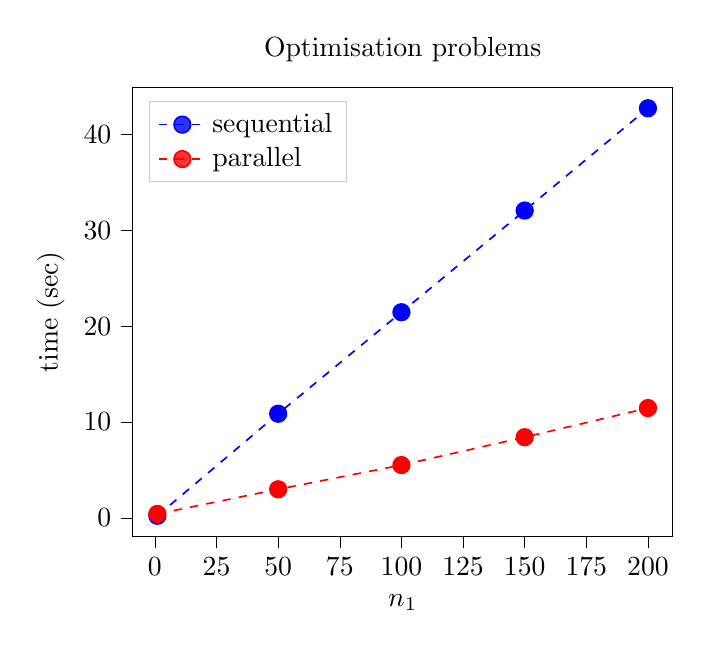
\begin{tikzpicture}

\begin{axis}[
legend cell align={left},
legend style={
  fill opacity=0.8,
  draw opacity=1,
  text opacity=1,
  at={(0.03,0.97)},
  anchor=north west,
  draw=white!80!black
},
tick align=outside,
tick pos=left,
title={Optimisation problems},
x grid style={white!69.0196078431373!black},
xlabel={\(\displaystyle n_1\)},
xmin=-8.95, xmax=209.95,
xtick style={color=black},
xtick={-25,0,25,50,75,100,125,150,175,200,225},
xticklabels={
  \(\displaystyle {\ensuremath{-}25}\),
  \(\displaystyle {0}\),
  \(\displaystyle {25}\),
  \(\displaystyle {50}\),
  \(\displaystyle {75}\),
  \(\displaystyle {100}\),
  \(\displaystyle {125}\),
  \(\displaystyle {150}\),
  \(\displaystyle {175}\),
  \(\displaystyle {200}\),
  \(\displaystyle {225}\)
},
y grid style={white!69.0196078431373!black},
ylabel={time (sec)},
ymin=-1.91896843149916, ymax=44.8788451695003,
ytick style={color=black},
ytick={-10,0,10,20,30,40,50},
yticklabels={
  \(\displaystyle {\ensuremath{-}10}\),
  \(\displaystyle {0}\),
  \(\displaystyle {10}\),
  \(\displaystyle {20}\),
  \(\displaystyle {30}\),
  \(\displaystyle {40}\),
  \(\displaystyle {50}\)
}
]
\addplot [semithick, blue, dashed, mark=*, mark size=3, mark options={solid}]
table {%
1 0.208204914000817
50 10.8651014509996
100 21.4615424589974
150 32.0731122189973
200 42.7516718240004
};
\addlegendentry{sequential}
\addplot [semithick, red, dashed, mark=*, mark size=3, mark options={solid}]
table {%
1 0.408692035001877
50 2.97865102099968
100 5.50569359699875
150 8.41258640300293
200 11.4589973489965
};
\addlegendentry{parallel}
\end{axis}

\end{tikzpicture}

    }
    \resizebox{.45\columnwidth}{!}{%
      \input{./latex_files/images/chapter4/exec_time_region.tex}
    }
    % \resizebox{.32\columnwidth}{!}{%
    %   % This file was created with tikzplotlib v0.9.12.
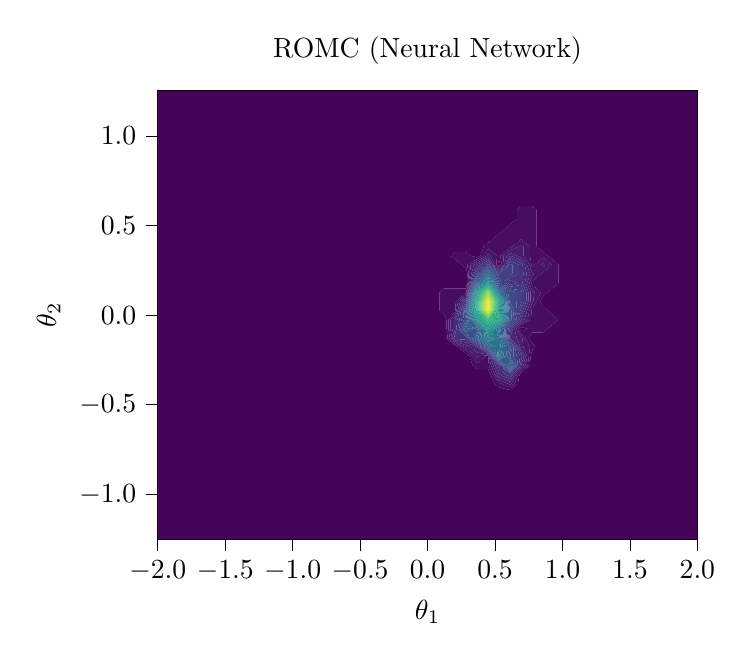
\begin{tikzpicture}

\definecolor{color0}{rgb}{0.269944,0.014625,0.341379}
\definecolor{color1}{rgb}{0.277018,0.050344,0.375715}
\definecolor{color2}{rgb}{0.281446,0.08432,0.407414}
\definecolor{color3}{rgb}{0.283197,0.11568,0.436115}
\definecolor{color4}{rgb}{0.28229,0.145912,0.46151}
\definecolor{color5}{rgb}{0.278826,0.17549,0.483397}
\definecolor{color6}{rgb}{0.274128,0.199721,0.498911}
\definecolor{color7}{rgb}{0.26658,0.228262,0.514349}
\definecolor{color8}{rgb}{0.257322,0.25613,0.526563}
\definecolor{color9}{rgb}{0.246811,0.283237,0.535941}
\definecolor{color10}{rgb}{0.235526,0.309527,0.542944}
\definecolor{color11}{rgb}{0.225863,0.330805,0.547314}
\definecolor{color12}{rgb}{0.214298,0.355619,0.551184}
\definecolor{color13}{rgb}{0.203063,0.379716,0.553925}
\definecolor{color14}{rgb}{0.192357,0.403199,0.555836}
\definecolor{color15}{rgb}{0.182256,0.426184,0.55712}
\definecolor{color16}{rgb}{0.172719,0.448791,0.557885}
\definecolor{color17}{rgb}{0.165117,0.467423,0.558141}
\definecolor{color18}{rgb}{0.15627,0.489624,0.557936}
\definecolor{color19}{rgb}{0.147607,0.511733,0.557049}
\definecolor{color20}{rgb}{0.139147,0.533812,0.555298}
\definecolor{color21}{rgb}{0.131172,0.555899,0.552459}
\definecolor{color22}{rgb}{0.125394,0.574318,0.549086}
\definecolor{color23}{rgb}{0.120565,0.596422,0.543611}
\definecolor{color24}{rgb}{0.119699,0.61849,0.536347}
\definecolor{color25}{rgb}{0.12478,0.640461,0.527068}
\definecolor{color26}{rgb}{0.137339,0.662252,0.515571}
\definecolor{color27}{rgb}{0.157851,0.683765,0.501686}
\definecolor{color28}{rgb}{0.180653,0.701402,0.488189}
\definecolor{color29}{rgb}{0.214,0.722114,0.469588}
\definecolor{color30}{rgb}{0.252899,0.742211,0.448284}
\definecolor{color31}{rgb}{0.296479,0.761561,0.424223}
\definecolor{color32}{rgb}{0.344074,0.780029,0.397381}
\definecolor{color33}{rgb}{0.386433,0.794644,0.372886}
\definecolor{color34}{rgb}{0.440137,0.811138,0.340967}
\definecolor{color35}{rgb}{0.496615,0.826376,0.306377}
\definecolor{color36}{rgb}{0.555484,0.840254,0.269281}
\definecolor{color37}{rgb}{0.616293,0.852709,0.230052}
\definecolor{color38}{rgb}{0.668054,0.861999,0.196293}
\definecolor{color39}{rgb}{0.730889,0.871916,0.156029}
\definecolor{color40}{rgb}{0.79376,0.880678,0.120005}
\definecolor{color41}{rgb}{0.85581,0.888601,0.097452}
\definecolor{color42}{rgb}{0.916242,0.896091,0.100717}
\definecolor{color43}{rgb}{0.974417,0.90359,0.130215}

\begin{axis}[
tick align=outside,
tick pos=left,
title={ROMC (Neural Network)},
x grid style={white!69.0196078431373!black},
xlabel={\(\displaystyle \theta_1\)},
xmin=-2, xmax=2,
xtick style={color=black},
xtick={-2,-1.5,-1,-0.5,0,0.5,1,1.5,2},
xticklabels={
  \(\displaystyle {\ensuremath{-}2.0}\),
  \(\displaystyle {\ensuremath{-}1.5}\),
  \(\displaystyle {\ensuremath{-}1.0}\),
  \(\displaystyle {\ensuremath{-}0.5}\),
  \(\displaystyle {0.0}\),
  \(\displaystyle {0.5}\),
  \(\displaystyle {1.0}\),
  \(\displaystyle {1.5}\),
  \(\displaystyle {2.0}\)
},
y grid style={white!69.0196078431373!black},
ylabel={\(\displaystyle \theta_2\)},
ymin=-1.25, ymax=1.25,
ytick style={color=black},
ytick={-1.5,-1,-0.5,0,0.5,1,1.5},
yticklabels={
  \(\displaystyle {\ensuremath{-}1.5}\),
  \(\displaystyle {\ensuremath{-}1.0}\),
  \(\displaystyle {\ensuremath{-}0.5}\),
  \(\displaystyle {0.0}\),
  \(\displaystyle {0.5}\),
  \(\displaystyle {1.0}\),
  \(\displaystyle {1.5}\)
}
]
\addplot [draw=none, fill=color0]
table{%
x  y
-1.91836734693878 -1.25
-1.83673469387755 -1.25
-1.75510204081633 -1.25
-1.6734693877551 -1.25
-1.59183673469388 -1.25
-1.51020408163265 -1.25
-1.42857142857143 -1.25
-1.3469387755102 -1.25
-1.26530612244898 -1.25
-1.18367346938776 -1.25
-1.10204081632653 -1.25
-1.02040816326531 -1.25
-0.938775510204082 -1.25
-0.857142857142857 -1.25
-0.775510204081633 -1.25
-0.693877551020408 -1.25
-0.612244897959184 -1.25
-0.530612244897959 -1.25
-0.448979591836735 -1.25
-0.36734693877551 -1.25
-0.285714285714286 -1.25
-0.204081632653061 -1.25
-0.122448979591837 -1.25
-0.0408163265306123 -1.25
0.0408163265306123 -1.25
0.122448979591836 -1.25
0.204081632653061 -1.25
0.285714285714286 -1.25
0.36734693877551 -1.25
0.448979591836734 -1.25
0.530612244897959 -1.25
0.612244897959183 -1.25
0.693877551020408 -1.25
0.775510204081633 -1.25
0.857142857142857 -1.25
0.938775510204081 -1.25
1.02040816326531 -1.25
1.10204081632653 -1.25
1.18367346938775 -1.25
1.26530612244898 -1.25
1.3469387755102 -1.25
1.42857142857143 -1.25
1.51020408163265 -1.25
1.59183673469388 -1.25
1.6734693877551 -1.25
1.75510204081633 -1.25
1.83673469387755 -1.25
1.91836734693878 -1.25
2 -1.25
2 -1.19897959183673
2 -1.14795918367347
2 -1.0969387755102
2 -1.04591836734694
2 -0.994897959183674
2 -0.943877551020408
2 -0.892857142857143
2 -0.841836734693878
2 -0.790816326530612
2 -0.739795918367347
2 -0.688775510204082
2 -0.637755102040816
2 -0.586734693877551
2 -0.535714285714286
2 -0.48469387755102
2 -0.433673469387755
2 -0.38265306122449
2 -0.331632653061224
2 -0.280612244897959
2 -0.229591836734694
2 -0.178571428571429
2 -0.127551020408163
2 -0.0765306122448979
2 -0.0255102040816326
2 0.0255102040816326
2 0.0765306122448979
2 0.127551020408163
2 0.178571428571429
2 0.229591836734694
2 0.280612244897959
2 0.331632653061225
2 0.38265306122449
2 0.433673469387755
2 0.48469387755102
2 0.535714285714286
2 0.586734693877551
2 0.637755102040816
2 0.688775510204082
2 0.739795918367347
2 0.790816326530612
2 0.841836734693878
2 0.892857142857143
2 0.943877551020408
2 0.994897959183674
2 1.04591836734694
2 1.0969387755102
2 1.14795918367347
2 1.19897959183673
2 1.25
1.91836734693878 1.25
1.83673469387755 1.25
1.75510204081633 1.25
1.6734693877551 1.25
1.59183673469388 1.25
1.51020408163265 1.25
1.42857142857143 1.25
1.3469387755102 1.25
1.26530612244898 1.25
1.18367346938775 1.25
1.10204081632653 1.25
1.02040816326531 1.25
0.938775510204081 1.25
0.857142857142857 1.25
0.775510204081633 1.25
0.693877551020408 1.25
0.612244897959183 1.25
0.530612244897959 1.25
0.448979591836734 1.25
0.36734693877551 1.25
0.285714285714286 1.25
0.204081632653061 1.25
0.122448979591836 1.25
0.0408163265306123 1.25
-0.0408163265306123 1.25
-0.122448979591837 1.25
-0.204081632653061 1.25
-0.285714285714286 1.25
-0.36734693877551 1.25
-0.448979591836735 1.25
-0.530612244897959 1.25
-0.612244897959184 1.25
-0.693877551020408 1.25
-0.775510204081633 1.25
-0.857142857142857 1.25
-0.938775510204082 1.25
-1.02040816326531 1.25
-1.10204081632653 1.25
-1.18367346938776 1.25
-1.26530612244898 1.25
-1.3469387755102 1.25
-1.42857142857143 1.25
-1.51020408163265 1.25
-1.59183673469388 1.25
-1.6734693877551 1.25
-1.75510204081633 1.25
-1.83673469387755 1.25
-1.91836734693878 1.25
-2 1.25
-2 1.19897959183673
-2 1.14795918367347
-2 1.0969387755102
-2 1.04591836734694
-2 0.994897959183674
-2 0.943877551020408
-2 0.892857142857143
-2 0.841836734693878
-2 0.790816326530612
-2 0.739795918367347
-2 0.688775510204082
-2 0.637755102040816
-2 0.586734693877551
-2 0.535714285714286
-2 0.48469387755102
-2 0.433673469387755
-2 0.38265306122449
-2 0.331632653061225
-2 0.280612244897959
-2 0.229591836734694
-2 0.178571428571429
-2 0.127551020408163
-2 0.0765306122448979
-2 0.0255102040816326
-2 -0.0255102040816326
-2 -0.0765306122448979
-2 -0.127551020408163
-2 -0.178571428571429
-2 -0.229591836734694
-2 -0.280612244897959
-2 -0.331632653061224
-2 -0.38265306122449
-2 -0.433673469387755
-2 -0.48469387755102
-2 -0.535714285714286
-2 -0.586734693877551
-2 -0.637755102040816
-2 -0.688775510204082
-2 -0.739795918367347
-2 -0.790816326530612
-2 -0.841836734693878
-2 -0.892857142857143
-2 -0.943877551020408
-2 -0.994897959183674
-2 -1.04591836734694
-2 -1.0969387755102
-2 -1.14795918367347
-2 -1.19897959183673
-2 -1.25
-1.91836734693878 -1.25

0.497959183673469 -0.38265306122449
0.465306122448979 -0.331632653061224
0.448979591836734 -0.301020408163265
0.36734693877551 -0.301020408163265
0.33469387755102 -0.280612244897959
0.310204081632653 -0.229591836734694
0.285714285714286 -0.214285714285714
0.228571428571428 -0.178571428571429
0.204081632653061 -0.170918367346939
0.13469387755102 -0.127551020408163
0.138775510204081 -0.0765306122448979
0.138775510204081 -0.0255102040816326
0.122448979591836 0.00510204081632653
0.0897959183673468 0.0255102040816326
0.0897959183673468 0.0765306122448979
0.0897959183673468 0.127551020408163
0.122448979591836 0.147959183673469
0.204081632653061 0.147959183673469
0.285714285714286 0.147959183673469
0.291836734693877 0.178571428571429
0.295510204081633 0.229591836734694
0.285714285714286 0.260204081632653
0.253061224489796 0.280612244897959
0.204081632653061 0.311224489795918
0.171428571428571 0.331632653061225
0.204081632653061 0.352040816326531
0.285714285714286 0.352040816326531
0.318367346938775 0.331632653061225
0.36734693877551 0.321428571428572
0.391836734693877 0.331632653061225
0.416326530612245 0.38265306122449
0.448979591836734 0.403061224489796
0.497959183673469 0.433673469387755
0.530612244897959 0.454081632653061
0.579591836734694 0.48469387755102
0.612244897959183 0.505102040816326
0.661224489795918 0.535714285714286
0.661224489795918 0.586734693877551
0.693877551020408 0.607142857142857
0.775510204081633 0.607142857142857
0.808163265306122 0.586734693877551
0.808163265306122 0.535714285714286
0.808163265306122 0.48469387755102
0.808163265306122 0.433673469387755
0.808163265306122 0.38265306122449
0.857142857142857 0.352040816326531
0.889795918367347 0.331632653061225
0.938775510204081 0.301020408163265
0.971428571428571 0.280612244897959
0.971428571428571 0.229591836734694
0.971428571428571 0.178571428571429
0.938775510204081 0.158163265306123
0.889795918367347 0.127551020408163
0.857142857142857 0.107142857142857
0.832653061224489 0.0765306122448979
0.857142857142857 0.0459183673469387
0.889795918367347 0.0255102040816326
0.938775510204081 -0.00510204081632653
0.971428571428571 -0.0255102040816326
0.938775510204081 -0.0459183673469387
0.889795918367347 -0.0765306122448979
0.857142857142857 -0.096938775510204
0.775510204081633 -0.096938775510204
0.751020408163265 -0.127551020408163
0.775510204081633 -0.158163265306122
0.808163265306122 -0.178571428571429
0.775510204081633 -0.198979591836735
0.763265306122449 -0.229591836734694
0.759183673469388 -0.280612244897959
0.693877551020408 -0.321428571428571
0.681632653061224 -0.331632653061224
0.669387755102041 -0.38265306122449
0.612244897959183 -0.418367346938776
0.530612244897959 -0.403061224489796
0.497959183673469 -0.38265306122449
};
\addplot [draw=none, fill=color0]
table{%
x  y
0.693877551020408 -0.0918367346938775
0.742857142857143 -0.0765306122448979
0.693877551020408 -0.0663265306122448
0.681632653061224 -0.0765306122448979
0.693877551020408 -0.0918367346938775
};
\addplot [draw=none, fill=color0]
table{%
x  y
0.530612244897959 0.274489795918367
0.540408163265306 0.280612244897959
0.530612244897959 0.311224489795918
0.520816326530612 0.280612244897959
0.530612244897959 0.274489795918367
};
\addplot [draw=none, fill=color1]
table{%
x  y
0.530612244897959 -0.403061224489796
0.612244897959183 -0.418367346938776
0.669387755102041 -0.38265306122449
0.681632653061224 -0.331632653061224
0.693877551020408 -0.321428571428571
0.759183673469388 -0.280612244897959
0.763265306122449 -0.229591836734694
0.775510204081633 -0.198979591836735
0.808163265306122 -0.178571428571429
0.775510204081633 -0.158163265306122
0.751020408163265 -0.127551020408163
0.775510204081633 -0.096938775510204
0.857142857142857 -0.096938775510204
0.889795918367347 -0.0765306122448979
0.938775510204081 -0.0459183673469387
0.971428571428571 -0.0255102040816326
0.938775510204081 -0.00510204081632653
0.889795918367347 0.0255102040816326
0.857142857142857 0.0459183673469387
0.832653061224489 0.0765306122448979
0.857142857142857 0.107142857142857
0.889795918367347 0.127551020408163
0.938775510204081 0.158163265306123
0.971428571428571 0.178571428571429
0.971428571428571 0.229591836734694
0.971428571428571 0.280612244897959
0.938775510204081 0.301020408163265
0.889795918367347 0.331632653061225
0.857142857142857 0.352040816326531
0.808163265306122 0.38265306122449
0.808163265306122 0.433673469387755
0.808163265306122 0.48469387755102
0.808163265306122 0.535714285714286
0.808163265306122 0.586734693877551
0.775510204081633 0.607142857142857
0.693877551020408 0.607142857142857
0.661224489795918 0.586734693877551
0.661224489795918 0.535714285714286
0.612244897959183 0.505102040816326
0.579591836734694 0.48469387755102
0.530612244897959 0.454081632653061
0.497959183673469 0.433673469387755
0.448979591836734 0.403061224489796
0.416326530612245 0.38265306122449
0.391836734693877 0.331632653061225
0.36734693877551 0.321428571428572
0.318367346938775 0.331632653061225
0.285714285714286 0.352040816326531
0.204081632653061 0.352040816326531
0.171428571428571 0.331632653061225
0.204081632653061 0.311224489795918
0.253061224489796 0.280612244897959
0.285714285714286 0.260204081632653
0.295510204081633 0.229591836734694
0.291836734693877 0.178571428571429
0.285714285714286 0.147959183673469
0.204081632653061 0.147959183673469
0.122448979591836 0.147959183673469
0.0897959183673468 0.127551020408163
0.0897959183673468 0.0765306122448979
0.0897959183673468 0.0255102040816326
0.122448979591836 0.00510204081632653
0.138775510204081 -0.0255102040816326
0.138775510204081 -0.0765306122448979
0.13469387755102 -0.127551020408163
0.204081632653061 -0.170918367346939
0.228571428571428 -0.178571428571429
0.285714285714286 -0.214285714285714
0.310204081632653 -0.229591836734694
0.33469387755102 -0.280612244897959
0.36734693877551 -0.301020408163265
0.448979591836734 -0.301020408163265
0.465306122448979 -0.331632653061224
0.497959183673469 -0.38265306122449
0.530612244897959 -0.403061224489796

0.546938775510204 -0.38265306122449
0.530612244897959 -0.377551020408163
0.481632653061224 -0.331632653061224
0.454421768707483 -0.280612244897959
0.450612244897959 -0.229591836734694
0.448979591836734 -0.228134110787172
0.432653061224489 -0.229591836734694
0.36734693877551 -0.270408163265306
0.33469387755102 -0.229591836734694
0.285714285714286 -0.198979591836735
0.253061224489796 -0.178571428571429
0.204081632653061 -0.163265306122449
0.146938775510204 -0.127551020408163
0.155102040816326 -0.0765306122448979
0.155102040816326 -0.0255102040816326
0.204081632653061 0.0204081632653061
0.206802721088435 0.0255102040816326
0.209523809523809 0.0765306122448979
0.285714285714286 0.124149659863946
0.286970172684458 0.127551020408163
0.297959183673469 0.178571428571429
0.305306122448979 0.229591836734694
0.293877551020408 0.280612244897959
0.36734693877551 0.311224489795918
0.416326530612245 0.331632653061225
0.448979591836734 0.372448979591837
0.514285714285714 0.331632653061225
0.511020408163265 0.280612244897959
0.530612244897959 0.268367346938776
0.550204081632653 0.280612244897959
0.538775510204081 0.331632653061225
0.612244897959183 0.377551020408163
0.628571428571428 0.38265306122449
0.693877551020408 0.423469387755102
0.759183673469388 0.38265306122449
0.759183673469388 0.331632653061225
0.770068027210884 0.280612244897959
0.775510204081633 0.270408163265306
0.791836734693877 0.280612244897959
0.857142857142857 0.321428571428572
0.922448979591836 0.280612244897959
0.857142857142857 0.239795918367347
0.840816326530612 0.229591836734694
0.775510204081633 0.188775510204082
0.770068027210884 0.178571428571429
0.775510204081633 0.168367346938776
0.840816326530612 0.127551020408163
0.808163265306122 0.0765306122448979
0.775510204081633 0.0357142857142857
0.770068027210884 0.0255102040816326
0.76734693877551 -0.0255102040816326
0.693877551020408 -0.0561224489795918
0.669387755102041 -0.0765306122448979
0.693877551020408 -0.107142857142857
0.726530612244898 -0.127551020408163
0.759183673469388 -0.178571428571429
0.751020408163265 -0.229591836734694
0.742857142857143 -0.280612244897959
0.693877551020408 -0.311224489795918
0.669387755102041 -0.331632653061224
0.644897959183673 -0.38265306122449
0.612244897959183 -0.403061224489796
0.546938775510204 -0.38265306122449

0.681632653061224 -0.0765306122448979
0.693877551020408 -0.0663265306122448
0.742857142857143 -0.0765306122448979
0.693877551020408 -0.0918367346938775
0.681632653061224 -0.0765306122448979

0.520816326530612 0.280612244897959
0.530612244897959 0.311224489795918
0.540408163265306 0.280612244897959
0.530612244897959 0.274489795918367
0.520816326530612 0.280612244897959
};
\addplot [draw=none, fill=color2]
table{%
x  y
0.612244897959183 -0.403061224489796
0.644897959183673 -0.38265306122449
0.669387755102041 -0.331632653061224
0.693877551020408 -0.311224489795918
0.742857142857143 -0.280612244897959
0.751020408163265 -0.229591836734694
0.759183673469388 -0.178571428571429
0.726530612244898 -0.127551020408163
0.693877551020408 -0.107142857142857
0.669387755102041 -0.0765306122448979
0.693877551020408 -0.0561224489795918
0.76734693877551 -0.0255102040816326
0.770068027210884 0.0255102040816326
0.775510204081633 0.0357142857142857
0.808163265306122 0.0765306122448979
0.840816326530612 0.127551020408163
0.775510204081633 0.168367346938776
0.770068027210884 0.178571428571429
0.775510204081633 0.188775510204082
0.840816326530612 0.229591836734694
0.857142857142857 0.239795918367347
0.922448979591836 0.280612244897959
0.857142857142857 0.321428571428572
0.791836734693877 0.280612244897959
0.775510204081633 0.270408163265306
0.770068027210884 0.280612244897959
0.759183673469388 0.331632653061225
0.759183673469388 0.38265306122449
0.693877551020408 0.423469387755102
0.628571428571428 0.38265306122449
0.612244897959183 0.377551020408163
0.538775510204081 0.331632653061225
0.550204081632653 0.280612244897959
0.530612244897959 0.268367346938776
0.511020408163265 0.280612244897959
0.514285714285714 0.331632653061225
0.448979591836734 0.372448979591837
0.416326530612245 0.331632653061225
0.36734693877551 0.311224489795918
0.293877551020408 0.280612244897959
0.305306122448979 0.229591836734694
0.297959183673469 0.178571428571429
0.286970172684458 0.127551020408163
0.285714285714286 0.124149659863946
0.209523809523809 0.0765306122448979
0.206802721088435 0.0255102040816326
0.204081632653061 0.0204081632653061
0.155102040816326 -0.0255102040816326
0.155102040816326 -0.0765306122448979
0.146938775510204 -0.127551020408163
0.204081632653061 -0.163265306122449
0.253061224489796 -0.178571428571429
0.285714285714286 -0.198979591836735
0.33469387755102 -0.229591836734694
0.36734693877551 -0.270408163265306
0.432653061224489 -0.229591836734694
0.448979591836734 -0.228134110787172
0.450612244897959 -0.229591836734694
0.454421768707483 -0.280612244897959
0.481632653061224 -0.331632653061224
0.530612244897959 -0.377551020408163
0.546938775510204 -0.38265306122449
0.612244897959183 -0.403061224489796

0.595918367346939 -0.38265306122449
0.530612244897959 -0.362244897959184
0.497959183673469 -0.331632653061224
0.470748299319728 -0.280612244897959
0.455510204081632 -0.229591836734694
0.448979591836734 -0.223760932944606
0.383673469387755 -0.229591836734694
0.36734693877551 -0.239795918367347
0.359183673469388 -0.229591836734694
0.285714285714286 -0.183673469387755
0.277551020408163 -0.178571428571429
0.204081632653061 -0.155612244897959
0.159183673469387 -0.127551020408163
0.171428571428571 -0.0765306122448979
0.171428571428571 -0.0255102040816326
0.204081632653061 0.00510204081632652
0.214965986394558 0.0255102040816326
0.225850340136054 0.0765306122448979
0.285714285714286 0.113945578231293
0.290737833594976 0.127551020408163
0.304081632653061 0.178571428571429
0.315102040816326 0.229591836734694
0.318367346938775 0.280612244897959
0.36734693877551 0.301020408163265
0.440816326530612 0.331632653061225
0.448979591836734 0.341836734693878
0.465306122448979 0.331632653061225
0.501224489795918 0.280612244897959
0.530612244897959 0.262244897959184
0.56 0.280612244897959
0.563265306122449 0.331632653061225
0.612244897959183 0.362244897959184
0.677551020408163 0.38265306122449
0.693877551020408 0.392857142857143
0.710204081632653 0.38265306122449
0.710204081632653 0.331632653061225
0.753741496598639 0.280612244897959
0.775510204081633 0.239795918367347
0.791836734693877 0.229591836734694
0.775510204081633 0.219387755102041
0.753741496598639 0.178571428571429
0.775510204081633 0.137755102040816
0.791836734693877 0.127551020408163
0.783673469387755 0.0765306122448979
0.775510204081633 0.0663265306122448
0.753741496598639 0.0255102040816326
0.742857142857143 -0.0255102040816326
0.693877551020408 -0.0459183673469387
0.657142857142857 -0.0765306122448979
0.693877551020408 -0.122448979591837
0.70204081632653 -0.127551020408163
0.710204081632653 -0.178571428571429
0.738775510204082 -0.229591836734694
0.726530612244898 -0.280612244897959
0.693877551020408 -0.301020408163265
0.657142857142857 -0.331632653061224
0.620408163265306 -0.38265306122449
0.612244897959183 -0.387755102040816
0.595918367346939 -0.38265306122449

0.840816326530612 0.280612244897959
0.857142857142857 0.290816326530612
0.873469387755102 0.280612244897959
0.857142857142857 0.270408163265306
0.840816326530612 0.280612244897959
};
\addplot [draw=none, fill=color3]
table{%
x  y
0.612244897959183 -0.387755102040816
0.620408163265306 -0.38265306122449
0.657142857142857 -0.331632653061224
0.693877551020408 -0.301020408163265
0.726530612244898 -0.280612244897959
0.738775510204082 -0.229591836734694
0.710204081632653 -0.178571428571429
0.70204081632653 -0.127551020408163
0.693877551020408 -0.122448979591837
0.657142857142857 -0.0765306122448979
0.693877551020408 -0.0459183673469387
0.742857142857143 -0.0255102040816326
0.753741496598639 0.0255102040816326
0.775510204081633 0.0663265306122448
0.783673469387755 0.0765306122448979
0.791836734693877 0.127551020408163
0.775510204081633 0.137755102040816
0.753741496598639 0.178571428571429
0.775510204081633 0.219387755102041
0.791836734693877 0.229591836734694
0.775510204081633 0.239795918367347
0.753741496598639 0.280612244897959
0.710204081632653 0.331632653061225
0.710204081632653 0.38265306122449
0.693877551020408 0.392857142857143
0.677551020408163 0.38265306122449
0.612244897959183 0.362244897959184
0.563265306122449 0.331632653061225
0.56 0.280612244897959
0.530612244897959 0.262244897959184
0.501224489795918 0.280612244897959
0.465306122448979 0.331632653061225
0.448979591836734 0.341836734693878
0.440816326530612 0.331632653061225
0.36734693877551 0.301020408163265
0.318367346938775 0.280612244897959
0.315102040816326 0.229591836734694
0.304081632653061 0.178571428571429
0.290737833594976 0.127551020408163
0.285714285714286 0.113945578231293
0.225850340136054 0.0765306122448979
0.214965986394558 0.0255102040816326
0.204081632653061 0.00510204081632652
0.171428571428571 -0.0255102040816326
0.171428571428571 -0.0765306122448979
0.159183673469387 -0.127551020408163
0.204081632653061 -0.155612244897959
0.277551020408163 -0.178571428571429
0.285714285714286 -0.183673469387755
0.359183673469388 -0.229591836734694
0.36734693877551 -0.239795918367347
0.383673469387755 -0.229591836734694
0.448979591836734 -0.223760932944606
0.455510204081632 -0.229591836734694
0.470748299319728 -0.280612244897959
0.497959183673469 -0.331632653061224
0.530612244897959 -0.362244897959184
0.595918367346939 -0.38265306122449
0.612244897959183 -0.387755102040816

0.514285714285714 -0.331632653061224
0.487074829931972 -0.280612244897959
0.460408163265306 -0.229591836734694
0.448979591836734 -0.219387755102041
0.36734693877551 -0.209183673469388
0.318367346938775 -0.178571428571429
0.285714285714286 -0.168367346938776
0.204081632653061 -0.147959183673469
0.171428571428571 -0.127551020408163
0.187755102040816 -0.0765306122448979
0.187755102040816 -0.0255102040816326
0.204081632653061 -0.0102040816326531
0.22312925170068 0.0255102040816326
0.242176870748299 0.0765306122448979
0.285714285714286 0.103741496598639
0.294505494505494 0.127551020408163
0.310204081632653 0.178571428571429
0.324897959183673 0.229591836734694
0.342857142857143 0.280612244897959
0.36734693877551 0.290816326530612
0.448979591836734 0.324829931972789
0.491428571428571 0.280612244897959
0.530612244897959 0.256122448979592
0.569795918367347 0.280612244897959
0.587755102040816 0.331632653061225
0.612244897959183 0.346938775510204
0.661224489795918 0.331632653061225
0.693877551020408 0.321428571428572
0.737414965986394 0.280612244897959
0.759183673469388 0.229591836734694
0.737414965986394 0.178571428571429
0.764625850340136 0.127551020408163
0.764625850340136 0.0765306122448979
0.737414965986394 0.0255102040816326
0.718367346938775 -0.0255102040816326
0.693877551020408 -0.0357142857142857
0.644897959183673 -0.0765306122448979
0.661224489795918 -0.127551020408163
0.68734693877551 -0.178571428571429
0.693877551020408 -0.188775510204082
0.726530612244898 -0.229591836734694
0.710204081632653 -0.280612244897959
0.693877551020408 -0.290816326530612
0.644897959183673 -0.331632653061224
0.612244897959183 -0.372448979591837
0.530612244897959 -0.346938775510204
0.514285714285714 -0.331632653061224
};
\addplot [draw=none, fill=color3]
table{%
x  y
0.857142857142857 0.270408163265306
0.873469387755102 0.280612244897959
0.857142857142857 0.290816326530612
0.840816326530612 0.280612244897959
0.857142857142857 0.270408163265306
};
\addplot [draw=none, fill=color4]
table{%
x  y
0.530612244897959 -0.346938775510204
0.612244897959183 -0.372448979591837
0.644897959183673 -0.331632653061224
0.693877551020408 -0.290816326530612
0.710204081632653 -0.280612244897959
0.726530612244898 -0.229591836734694
0.693877551020408 -0.188775510204082
0.68734693877551 -0.178571428571429
0.661224489795918 -0.127551020408163
0.644897959183673 -0.0765306122448979
0.693877551020408 -0.0357142857142857
0.718367346938775 -0.0255102040816326
0.737414965986394 0.0255102040816326
0.764625850340136 0.0765306122448979
0.764625850340136 0.127551020408163
0.737414965986394 0.178571428571429
0.759183673469388 0.229591836734694
0.737414965986394 0.280612244897959
0.693877551020408 0.321428571428572
0.661224489795918 0.331632653061225
0.612244897959183 0.346938775510204
0.587755102040816 0.331632653061225
0.569795918367347 0.280612244897959
0.530612244897959 0.256122448979592
0.491428571428571 0.280612244897959
0.448979591836734 0.324829931972789
0.36734693877551 0.290816326530612
0.342857142857143 0.280612244897959
0.324897959183673 0.229591836734694
0.310204081632653 0.178571428571429
0.294505494505494 0.127551020408163
0.285714285714286 0.103741496598639
0.242176870748299 0.0765306122448979
0.22312925170068 0.0255102040816326
0.204081632653061 -0.0102040816326531
0.187755102040816 -0.0255102040816326
0.187755102040816 -0.0765306122448979
0.171428571428571 -0.127551020408163
0.204081632653061 -0.147959183673469
0.285714285714286 -0.168367346938776
0.318367346938775 -0.178571428571429
0.36734693877551 -0.209183673469388
0.448979591836734 -0.219387755102041
0.460408163265306 -0.229591836734694
0.487074829931972 -0.280612244897959
0.514285714285714 -0.331632653061224
0.530612244897959 -0.346938775510204

0.530612244897959 -0.331632653061224
0.530612244897959 -0.331632653061224
0.503401360544217 -0.280612244897959
0.465306122448979 -0.229591836734694
0.448979591836734 -0.215014577259475
0.36734693877551 -0.178571428571429
0.285714285714286 -0.153061224489796
0.204081632653061 -0.140306122448979
0.183673469387755 -0.127551020408163
0.204081632653061 -0.0765306122448979
0.204081632653061 -0.0765306122448979
0.204081632653061 -0.0255102040816326
0.231292517006803 0.0255102040816326
0.258503401360544 0.0765306122448979
0.285714285714286 0.0935374149659864
0.298273155416012 0.127551020408163
0.316326530612245 0.178571428571429
0.33469387755102 0.229591836734694
0.36734693877551 0.280612244897959
0.36734693877551 0.280612244897959
0.448979591836734 0.314625850340136
0.481632653061224 0.280612244897959
0.530612244897959 0.25
0.579591836734694 0.280612244897959
0.612244897959183 0.331632653061225
0.693877551020408 0.306122448979592
0.72108843537415 0.280612244897959
0.73469387755102 0.229591836734694
0.72108843537415 0.178571428571429
0.748299319727891 0.127551020408163
0.748299319727891 0.0765306122448979
0.72108843537415 0.0255102040816326
0.693877551020408 -0.0255102040816326
0.693877551020408 -0.0255102040816326
0.63265306122449 -0.0765306122448979
0.612244897959183 -0.127551020408163
0.612244897959183 -0.127551020408163
0.612244897959183 -0.127551020408163
0.677551020408163 -0.178571428571429
0.693877551020408 -0.204081632653061
0.714285714285714 -0.229591836734694
0.693877551020408 -0.280612244897959
0.693877551020408 -0.280612244897959
0.63265306122449 -0.331632653061224
0.612244897959183 -0.357142857142857
0.530612244897959 -0.331632653061224
};
\addplot [draw=none, fill=color4]
table{%
x  y
0.612244897959183 0.178571428571429
0.612244897959184 0.178571428571429
0.612244897959183 0.178571428571429
0.612244897959183 0.178571428571429
0.612244897959183 0.178571428571429
};
\addplot [draw=none, fill=color5]
table{%
x  y
0.612244897959183 -0.357142857142857
0.63265306122449 -0.331632653061224
0.693877551020408 -0.280612244897959
0.714285714285714 -0.229591836734694
0.693877551020408 -0.204081632653061
0.677551020408163 -0.178571428571429
0.612244897959183 -0.127551020408163
0.612244897959183 -0.127551020408163
0.63265306122449 -0.0765306122448979
0.693877551020408 -0.0255102040816326
0.693877551020408 -0.0255102040816326
0.72108843537415 0.0255102040816326
0.748299319727891 0.0765306122448979
0.748299319727891 0.127551020408163
0.72108843537415 0.178571428571429
0.73469387755102 0.229591836734694
0.72108843537415 0.280612244897959
0.693877551020408 0.306122448979592
0.612244897959183 0.331632653061225
0.579591836734694 0.280612244897959
0.530612244897959 0.25
0.481632653061224 0.280612244897959
0.448979591836734 0.314625850340136
0.36734693877551 0.280612244897959
0.36734693877551 0.280612244897959
0.33469387755102 0.229591836734694
0.316326530612245 0.178571428571429
0.298273155416012 0.127551020408163
0.285714285714286 0.0935374149659864
0.258503401360544 0.0765306122448979
0.231292517006803 0.0255102040816326
0.204081632653061 -0.0255102040816326
0.204081632653061 -0.0765306122448979
0.204081632653061 -0.0765306122448979
0.183673469387755 -0.127551020408163
0.204081632653061 -0.140306122448979
0.285714285714286 -0.153061224489796
0.36734693877551 -0.178571428571429
0.36734693877551 -0.178571428571429
0.448979591836734 -0.215014577259475
0.465306122448979 -0.229591836734694
0.503401360544217 -0.280612244897959
0.530612244897959 -0.331632653061224
0.530612244897959 -0.331632653061224
0.612244897959183 -0.357142857142857

0.579591836734694 -0.331632653061224
0.530612244897959 -0.301020408163265
0.519727891156462 -0.280612244897959
0.470204081632653 -0.229591836734694
0.448979591836734 -0.21064139941691
0.377142857142857 -0.178571428571429
0.36734693877551 -0.172448979591837
0.285714285714286 -0.137755102040816
0.204081632653061 -0.13265306122449
0.195918367346939 -0.127551020408163
0.204081632653061 -0.107142857142857
0.213877551020408 -0.0765306122448979
0.220408163265306 -0.0255102040816326
0.239455782312925 0.0255102040816326
0.274829931972789 0.0765306122448979
0.285714285714286 0.0833333333333333
0.302040816326531 0.127551020408163
0.322448979591837 0.178571428571429
0.344489795918367 0.229591836734694
0.36734693877551 0.26530612244898
0.391836734693877 0.280612244897959
0.448979591836734 0.304421768707483
0.471836734693877 0.280612244897959
0.530612244897959 0.243877551020408
0.589387755102041 0.280612244897959
0.612244897959183 0.316326530612245
0.693877551020408 0.290816326530612
0.704761904761905 0.280612244897959
0.710204081632653 0.229591836734694
0.704761904761905 0.178571428571429
0.731972789115646 0.127551020408163
0.731972789115646 0.0765306122448979
0.704761904761905 0.0255102040816326
0.693877551020408 0.00510204081632655
0.681632653061224 -0.0255102040816326
0.620408163265306 -0.0765306122448979
0.612244897959183 -0.0969387755102039
0.605247813411079 -0.127551020408163
0.612244897959183 -0.135204081632653
0.667755102040816 -0.178571428571429
0.693877551020408 -0.219387755102041
0.70204081632653 -0.229591836734694
0.693877551020408 -0.25
0.685714285714286 -0.280612244897959
0.620408163265306 -0.331632653061224
0.612244897959183 -0.341836734693878
0.579591836734694 -0.331632653061224
};
\addplot [draw=none, fill=color5]
table{%
x  y
0.612244897959183 0.168367346938776
0.661224489795918 0.178571428571429
0.612244897959183 0.193877551020408
0.595918367346938 0.178571428571429
0.612244897959183 0.168367346938776

0.612244897959183 0.178571428571429
0.612244897959183 0.178571428571429
0.612244897959184 0.178571428571429
0.612244897959183 0.178571428571429
0.612244897959183 0.178571428571429
};
\addplot [draw=none, fill=color6]
table{%
x  y
0.612244897959183 -0.341836734693878
0.620408163265306 -0.331632653061224
0.685714285714286 -0.280612244897959
0.693877551020408 -0.25
0.70204081632653 -0.229591836734694
0.693877551020408 -0.219387755102041
0.667755102040816 -0.178571428571429
0.612244897959183 -0.135204081632653
0.605247813411078 -0.127551020408163
0.612244897959183 -0.0969387755102039
0.620408163265306 -0.0765306122448979
0.681632653061224 -0.0255102040816326
0.693877551020408 0.00510204081632655
0.704761904761905 0.0255102040816326
0.731972789115646 0.0765306122448979
0.731972789115646 0.127551020408163
0.704761904761905 0.178571428571429
0.710204081632653 0.229591836734694
0.704761904761905 0.280612244897959
0.693877551020408 0.290816326530612
0.612244897959183 0.316326530612245
0.589387755102041 0.280612244897959
0.530612244897959 0.243877551020408
0.471836734693877 0.280612244897959
0.448979591836734 0.304421768707483
0.391836734693877 0.280612244897959
0.36734693877551 0.26530612244898
0.344489795918367 0.229591836734694
0.322448979591837 0.178571428571429
0.302040816326531 0.127551020408163
0.285714285714286 0.0833333333333333
0.274829931972789 0.0765306122448979
0.239455782312925 0.0255102040816326
0.220408163265306 -0.0255102040816326
0.213877551020408 -0.0765306122448979
0.204081632653061 -0.107142857142857
0.195918367346939 -0.127551020408163
0.204081632653061 -0.13265306122449
0.285714285714286 -0.137755102040816
0.36734693877551 -0.172448979591837
0.377142857142857 -0.178571428571429
0.448979591836734 -0.21064139941691
0.470204081632653 -0.229591836734694
0.519727891156462 -0.280612244897959
0.530612244897959 -0.301020408163265
0.579591836734694 -0.331632653061224
0.612244897959183 -0.341836734693878

0.533877551020408 -0.280612244897959
0.530612244897959 -0.279154518950437
0.475102040816326 -0.229591836734694
0.448979591836734 -0.206268221574344
0.386938775510204 -0.178571428571429
0.36734693877551 -0.166326530612245
0.289795918367347 -0.127551020408163
0.285714285714286 -0.125
0.223673469387755 -0.0765306122448979
0.236734693877551 -0.0255102040816326
0.247619047619047 0.0255102040816326
0.285714285714286 0.0731292517006802
0.287074829931973 0.0765306122448979
0.305808477237049 0.127551020408163
0.328571428571429 0.178571428571429
0.354285714285714 0.229591836734694
0.36734693877551 0.25
0.416326530612245 0.280612244897959
0.448979591836734 0.29421768707483
0.46204081632653 0.280612244897959
0.530612244897959 0.237755102040816
0.599183673469388 0.280612244897959
0.612244897959183 0.301020408163265
0.677551020408163 0.280612244897959
0.677551020408163 0.229591836734694
0.612244897959183 0.209183673469388
0.579591836734694 0.178571428571429
0.612244897959183 0.158163265306122
0.693877551020408 0.168367346938775
0.715646258503401 0.127551020408163
0.715646258503401 0.0765306122448979
0.693877551020408 0.0357142857142857
0.68843537414966 0.0255102040816326
0.669387755102041 -0.0255102040816326
0.612244897959183 -0.0731292517006802
0.608979591836734 -0.0765306122448979
0.598250728862973 -0.127551020408163
0.612244897959183 -0.142857142857143
0.657959183673469 -0.178571428571429
0.685714285714285 -0.229591836734694
0.677551020408163 -0.280612244897959
0.612244897959183 -0.329591836734694
0.533877551020408 -0.280612244897959

0.595918367346938 0.178571428571429
0.612244897959183 0.193877551020408
0.661224489795918 0.178571428571429
0.612244897959183 0.168367346938776
0.595918367346938 0.178571428571429
};
\addplot [draw=none, fill=color7]
table{%
x  y
0.612244897959183 -0.329591836734694
0.677551020408163 -0.280612244897959
0.685714285714285 -0.229591836734694
0.657959183673469 -0.178571428571429
0.612244897959183 -0.142857142857143
0.598250728862973 -0.127551020408163
0.608979591836734 -0.0765306122448979
0.612244897959183 -0.0731292517006802
0.669387755102041 -0.0255102040816326
0.68843537414966 0.0255102040816326
0.693877551020408 0.0357142857142857
0.715646258503401 0.0765306122448979
0.715646258503401 0.127551020408163
0.693877551020408 0.168367346938775
0.612244897959183 0.158163265306122
0.579591836734694 0.178571428571429
0.612244897959183 0.209183673469388
0.677551020408163 0.229591836734694
0.677551020408163 0.280612244897959
0.612244897959183 0.301020408163265
0.599183673469388 0.280612244897959
0.530612244897959 0.237755102040816
0.46204081632653 0.280612244897959
0.448979591836734 0.29421768707483
0.416326530612245 0.280612244897959
0.36734693877551 0.25
0.354285714285714 0.229591836734694
0.328571428571429 0.178571428571429
0.305808477237049 0.127551020408163
0.287074829931973 0.0765306122448979
0.285714285714286 0.0731292517006802
0.247619047619047 0.0255102040816326
0.236734693877551 -0.0255102040816326
0.223673469387755 -0.0765306122448979
0.285714285714286 -0.125
0.289795918367347 -0.127551020408163
0.36734693877551 -0.166326530612245
0.386938775510204 -0.178571428571429
0.448979591836734 -0.206268221574344
0.475102040816326 -0.229591836734694
0.530612244897959 -0.279154518950437
0.533877551020408 -0.280612244897959
0.612244897959183 -0.329591836734694

0.543673469387755 -0.280612244897959
0.530612244897959 -0.274781341107872
0.48 -0.229591836734694
0.448979591836734 -0.201895043731778
0.396734693877551 -0.178571428571429
0.36734693877551 -0.160204081632653
0.302040816326531 -0.127551020408163
0.285714285714286 -0.11734693877551
0.233469387755102 -0.0765306122448979
0.253061224489796 -0.0255102040816326
0.25578231292517 0.0255102040816326
0.285714285714286 0.0629251700680271
0.291156462585034 0.0765306122448979
0.309576138147567 0.127551020408163
0.33469387755102 0.178571428571429
0.364081632653061 0.229591836734694
0.36734693877551 0.23469387755102
0.440816326530612 0.280612244897959
0.448979591836734 0.284013605442177
0.452244897959183 0.280612244897959
0.530612244897959 0.231632653061224
0.608979591836735 0.280612244897959
0.612244897959183 0.285714285714286
0.628571428571428 0.280612244897959
0.628571428571428 0.229591836734694
0.612244897959183 0.224489795918367
0.563265306122449 0.178571428571429
0.612244897959183 0.147959183673469
0.693877551020408 0.137755102040816
0.699319727891156 0.127551020408163
0.699319727891156 0.0765306122448979
0.693877551020408 0.0663265306122449
0.672108843537415 0.0255102040816326
0.657142857142857 -0.0255102040816326
0.612244897959183 -0.0629251700680271
0.599183673469388 -0.0765306122448979
0.591253644314869 -0.127551020408163
0.612244897959183 -0.150510204081633
0.648163265306122 -0.178571428571429
0.661224489795918 -0.229591836734694
0.669387755102041 -0.280612244897959
0.612244897959183 -0.323469387755102
0.543673469387755 -0.280612244897959
};
\addplot [draw=none, fill=color8]
table{%
x  y
0.612244897959183 -0.323469387755102
0.669387755102041 -0.280612244897959
0.661224489795918 -0.229591836734694
0.648163265306122 -0.178571428571429
0.612244897959183 -0.150510204081633
0.591253644314869 -0.127551020408163
0.599183673469388 -0.0765306122448979
0.612244897959183 -0.0629251700680271
0.657142857142857 -0.0255102040816326
0.672108843537415 0.0255102040816326
0.693877551020408 0.0663265306122449
0.699319727891156 0.0765306122448979
0.699319727891156 0.127551020408163
0.693877551020408 0.137755102040816
0.612244897959183 0.147959183673469
0.563265306122449 0.178571428571429
0.612244897959183 0.224489795918367
0.628571428571428 0.229591836734694
0.628571428571428 0.280612244897959
0.612244897959183 0.285714285714286
0.608979591836735 0.280612244897959
0.530612244897959 0.231632653061224
0.452244897959183 0.280612244897959
0.448979591836734 0.284013605442177
0.440816326530612 0.280612244897959
0.36734693877551 0.23469387755102
0.364081632653061 0.229591836734694
0.33469387755102 0.178571428571429
0.309576138147567 0.127551020408163
0.291156462585034 0.0765306122448979
0.285714285714286 0.0629251700680271
0.25578231292517 0.0255102040816326
0.253061224489796 -0.0255102040816326
0.233469387755102 -0.0765306122448979
0.285714285714286 -0.11734693877551
0.302040816326531 -0.127551020408163
0.36734693877551 -0.160204081632653
0.396734693877551 -0.178571428571429
0.448979591836734 -0.201895043731778
0.48 -0.229591836734694
0.530612244897959 -0.274781341107872
0.543673469387755 -0.280612244897959
0.612244897959183 -0.323469387755102

0.553469387755102 -0.280612244897959
0.530612244897959 -0.270408163265306
0.484897959183673 -0.229591836734694
0.448979591836734 -0.197521865889213
0.406530612244898 -0.178571428571429
0.36734693877551 -0.154081632653061
0.314285714285714 -0.127551020408163
0.285714285714286 -0.10969387755102
0.243265306122449 -0.0765306122448979
0.269387755102041 -0.0255102040816326
0.263945578231292 0.0255102040816326
0.285714285714286 0.0527210884353741
0.295238095238095 0.0765306122448979
0.313343799058085 0.127551020408163
0.340816326530612 0.178571428571429
0.36734693877551 0.222789115646258
0.375510204081633 0.229591836734694
0.448979591836734 0.275510204081633
0.522448979591836 0.229591836734694
0.530612244897959 0.209183673469388
0.546938775510204 0.178571428571429
0.612244897959183 0.137755102040816
0.661224489795918 0.127551020408163
0.661224489795918 0.0765306122448979
0.65578231292517 0.0255102040816326
0.644897959183673 -0.0255102040816326
0.612244897959183 -0.0527210884353741
0.589387755102041 -0.0765306122448979
0.584256559766764 -0.127551020408163
0.612244897959183 -0.158163265306122
0.638367346938775 -0.178571428571429
0.636734693877551 -0.229591836734694
0.661224489795918 -0.280612244897959
0.612244897959183 -0.31734693877551
0.553469387755102 -0.280612244897959
};
\addplot [draw=none, fill=color9]
table{%
x  y
0.612244897959183 -0.31734693877551
0.661224489795918 -0.280612244897959
0.636734693877551 -0.229591836734694
0.638367346938775 -0.178571428571429
0.612244897959183 -0.158163265306122
0.584256559766764 -0.127551020408163
0.589387755102041 -0.0765306122448979
0.612244897959183 -0.0527210884353741
0.644897959183673 -0.0255102040816326
0.65578231292517 0.0255102040816326
0.661224489795918 0.0765306122448979
0.661224489795918 0.127551020408163
0.612244897959183 0.137755102040816
0.546938775510204 0.178571428571429
0.530612244897959 0.209183673469388
0.522448979591836 0.229591836734694
0.448979591836734 0.275510204081633
0.375510204081633 0.229591836734694
0.36734693877551 0.222789115646258
0.340816326530612 0.178571428571429
0.313343799058085 0.127551020408163
0.295238095238095 0.0765306122448979
0.285714285714286 0.0527210884353741
0.263945578231292 0.0255102040816326
0.269387755102041 -0.0255102040816326
0.243265306122449 -0.0765306122448979
0.285714285714286 -0.10969387755102
0.314285714285714 -0.127551020408163
0.36734693877551 -0.154081632653061
0.406530612244898 -0.178571428571429
0.448979591836734 -0.197521865889213
0.484897959183673 -0.229591836734694
0.530612244897959 -0.270408163265306
0.553469387755102 -0.280612244897959
0.612244897959183 -0.31734693877551

0.563265306122449 -0.280612244897959
0.530612244897959 -0.26603498542274
0.489795918367347 -0.229591836734694
0.448979591836734 -0.193148688046647
0.416326530612245 -0.178571428571429
0.36734693877551 -0.147959183673469
0.326530612244898 -0.127551020408163
0.285714285714286 -0.10204081632653
0.253061224489796 -0.0765306122448979
0.285714285714286 -0.0255102040816327
0.285714285714286 -0.0255102040816326
0.285714285714286 -0.0255102040816326
0.272108843537415 0.0255102040816326
0.285714285714286 0.042517006802721
0.299319727891156 0.0765306122448979
0.317111459968603 0.127551020408163
0.346938775510204 0.178571428571429
0.36734693877551 0.212585034013605
0.387755102040816 0.229591836734694
0.448979591836734 0.267857142857143
0.510204081632653 0.229591836734694
0.530612244897959 0.178571428571429
0.530612244897959 0.178571428571429
0.612244897959183 0.127551020408163
0.612244897959183 0.0765306122448979
0.612244897959183 0.0765306122448978
0.639455782312925 0.0255102040816326
0.63265306122449 -0.0255102040816326
0.612244897959183 -0.042517006802721
0.579591836734694 -0.0765306122448979
0.577259475218659 -0.127551020408163
0.612244897959183 -0.165816326530612
0.628571428571428 -0.178571428571429
0.612244897959183 -0.229591836734694
0.612244897959183 -0.229591836734694
0.653061224489796 -0.280612244897959
0.612244897959183 -0.311224489795918
0.563265306122449 -0.280612244897959
};
\addplot [draw=none, fill=color9]
table{%
x  y
0.36734693877551 -0.0765306122448979
0.36734693877551 -0.0765306122448979
0.36734693877551 -0.0765306122448979
0.36734693877551 -0.0765306122448979
0.36734693877551 -0.0765306122448979
};
\addplot [draw=none, fill=color10]
table{%
x  y
0.612244897959183 -0.311224489795918
0.653061224489796 -0.280612244897959
0.612244897959183 -0.229591836734694
0.612244897959183 -0.229591836734694
0.628571428571428 -0.178571428571429
0.612244897959183 -0.165816326530612
0.577259475218659 -0.127551020408163
0.579591836734694 -0.0765306122448979
0.612244897959183 -0.042517006802721
0.63265306122449 -0.0255102040816326
0.639455782312925 0.0255102040816326
0.612244897959183 0.0765306122448978
0.612244897959183 0.0765306122448979
0.612244897959183 0.127551020408163
0.530612244897959 0.178571428571429
0.530612244897959 0.178571428571429
0.510204081632653 0.229591836734694
0.448979591836734 0.267857142857143
0.387755102040816 0.229591836734694
0.36734693877551 0.212585034013605
0.346938775510204 0.178571428571429
0.317111459968603 0.127551020408163
0.299319727891156 0.0765306122448979
0.285714285714286 0.042517006802721
0.272108843537415 0.0255102040816326
0.285714285714286 -0.0255102040816326
0.285714285714286 -0.0255102040816326
0.285714285714286 -0.0255102040816327
0.253061224489796 -0.0765306122448979
0.285714285714286 -0.10204081632653
0.326530612244898 -0.127551020408163
0.36734693877551 -0.147959183673469
0.416326530612245 -0.178571428571429
0.448979591836734 -0.193148688046647
0.489795918367347 -0.229591836734694
0.530612244897959 -0.26603498542274
0.563265306122449 -0.280612244897959
0.612244897959183 -0.311224489795918

0.573061224489796 -0.280612244897959
0.530612244897959 -0.261661807580175
0.49469387755102 -0.229591836734694
0.448979591836734 -0.188775510204082
0.426122448979592 -0.178571428571429
0.36734693877551 -0.141836734693877
0.338775510204082 -0.127551020408163
0.36734693877551 -0.0918367346938775
0.373469387755102 -0.0765306122448979
0.36734693877551 -0.0721574344023323
0.342857142857143 -0.0765306122448979
0.285714285714286 -0.0943877551020407
0.262857142857143 -0.0765306122448979
0.285714285714286 -0.0408163265306122
0.292711370262391 -0.0255102040816326
0.285714285714286 0.0051020408163266
0.280272108843537 0.0255102040816326
0.285714285714286 0.032312925170068
0.303401360544218 0.0765306122448979
0.320879120879121 0.127551020408163
0.353061224489796 0.178571428571429
0.36734693877551 0.202380952380952
0.4 0.229591836734694
0.448979591836734 0.260204081632653
0.497959183673469 0.229591836734694
0.523615160349854 0.178571428571429
0.530612244897959 0.168367346938776
0.595918367346938 0.127551020408163
0.606802721088435 0.0765306122448979
0.612244897959183 0.0459183673469387
0.62312925170068 0.0255102040816326
0.620408163265306 -0.0255102040816326
0.612244897959183 -0.032312925170068
0.569795918367347 -0.0765306122448979
0.570262390670554 -0.127551020408163
0.612244897959183 -0.173469387755102
0.618775510204081 -0.178571428571429
0.612244897959183 -0.198979591836735
0.602448979591836 -0.229591836734694
0.612244897959183 -0.239795918367347
0.644897959183673 -0.280612244897959
0.612244897959183 -0.305102040816326
0.573061224489796 -0.280612244897959

0.36734693877551 -0.0765306122448979
0.36734693877551 -0.0765306122448979
0.36734693877551 -0.0765306122448979
0.36734693877551 -0.0765306122448979
0.36734693877551 -0.0765306122448979
};
\addplot [draw=none, fill=color11]
table{%
x  y
0.612244897959183 -0.305102040816326
0.644897959183673 -0.280612244897959
0.612244897959183 -0.239795918367347
0.602448979591836 -0.229591836734694
0.612244897959183 -0.198979591836735
0.618775510204081 -0.178571428571429
0.612244897959183 -0.173469387755102
0.570262390670554 -0.127551020408163
0.569795918367347 -0.0765306122448979
0.612244897959183 -0.032312925170068
0.620408163265306 -0.0255102040816326
0.62312925170068 0.0255102040816326
0.612244897959183 0.0459183673469387
0.606802721088435 0.0765306122448979
0.595918367346939 0.127551020408163
0.530612244897959 0.168367346938776
0.523615160349854 0.178571428571429
0.497959183673469 0.229591836734694
0.448979591836734 0.260204081632653
0.4 0.229591836734694
0.36734693877551 0.202380952380952
0.353061224489796 0.178571428571429
0.320879120879121 0.127551020408163
0.303401360544218 0.0765306122448979
0.285714285714286 0.032312925170068
0.280272108843537 0.0255102040816326
0.285714285714286 0.0051020408163266
0.292711370262391 -0.0255102040816326
0.285714285714286 -0.0408163265306122
0.262857142857143 -0.0765306122448979
0.285714285714286 -0.0943877551020407
0.342857142857143 -0.0765306122448979
0.36734693877551 -0.0721574344023323
0.373469387755102 -0.0765306122448979
0.36734693877551 -0.0918367346938775
0.338775510204082 -0.127551020408163
0.36734693877551 -0.141836734693877
0.426122448979592 -0.178571428571429
0.448979591836734 -0.188775510204082
0.49469387755102 -0.229591836734694
0.530612244897959 -0.261661807580175
0.573061224489796 -0.280612244897959
0.612244897959183 -0.305102040816326

0.582857142857143 -0.280612244897959
0.530612244897959 -0.257288629737609
0.499591836734694 -0.229591836734694
0.448979591836734 -0.184402332361516
0.435918367346938 -0.178571428571429
0.36734693877551 -0.135714285714286
0.351020408163265 -0.127551020408163
0.36734693877551 -0.107142857142857
0.379591836734694 -0.0765306122448979
0.36734693877551 -0.0677842565597667
0.318367346938775 -0.0765306122448979
0.285714285714286 -0.0867346938775509
0.27265306122449 -0.0765306122448979
0.285714285714286 -0.0561224489795918
0.299708454810496 -0.0255102040816326
0.287528344671202 0.0255102040816326
0.307482993197279 0.0765306122448979
0.324646781789639 0.127551020408163
0.359183673469388 0.178571428571429
0.36734693877551 0.192176870748299
0.412244897959184 0.229591836734694
0.448979591836734 0.252551020408163
0.485714285714285 0.229591836734694
0.516618075801749 0.178571428571429
0.530612244897959 0.158163265306122
0.579591836734694 0.127551020408163
0.601360544217687 0.0765306122448979
0.609523809523809 0.0255102040816326
0.610430839002267 -0.0255102040816326
0.56 -0.0765306122448979
0.563265306122449 -0.127551020408163
0.606802721088435 -0.178571428571429
0.59265306122449 -0.229591836734694
0.612244897959183 -0.25
0.636734693877551 -0.280612244897959
0.612244897959183 -0.298979591836735
0.582857142857143 -0.280612244897959
};
\addplot [draw=none, fill=color12]
table{%
x  y
0.612244897959183 -0.298979591836735
0.636734693877551 -0.280612244897959
0.612244897959183 -0.25
0.59265306122449 -0.229591836734694
0.606802721088435 -0.178571428571429
0.563265306122449 -0.127551020408163
0.56 -0.0765306122448979
0.610430839002267 -0.0255102040816326
0.609523809523809 0.0255102040816326
0.601360544217687 0.0765306122448979
0.579591836734694 0.127551020408163
0.530612244897959 0.158163265306122
0.516618075801749 0.178571428571429
0.485714285714285 0.229591836734694
0.448979591836734 0.252551020408163
0.412244897959184 0.229591836734694
0.36734693877551 0.192176870748299
0.359183673469388 0.178571428571429
0.324646781789639 0.127551020408163
0.307482993197279 0.0765306122448979
0.287528344671202 0.0255102040816326
0.299708454810496 -0.0255102040816326
0.285714285714286 -0.0561224489795918
0.27265306122449 -0.0765306122448979
0.285714285714286 -0.0867346938775509
0.318367346938775 -0.0765306122448979
0.36734693877551 -0.0677842565597667
0.379591836734694 -0.0765306122448979
0.36734693877551 -0.107142857142857
0.351020408163265 -0.127551020408163
0.36734693877551 -0.135714285714286
0.435918367346939 -0.178571428571429
0.448979591836734 -0.184402332361516
0.499591836734694 -0.229591836734694
0.530612244897959 -0.257288629737609
0.582857142857143 -0.280612244897959
0.612244897959183 -0.298979591836735

0.59265306122449 -0.280612244897959
0.612244897959183 -0.260204081632653
0.628571428571428 -0.280612244897959
0.612244897959183 -0.292857142857143
0.59265306122449 -0.280612244897959

0.504489795918367 -0.229591836734694
0.448979591836734 -0.18002915451895
0.445714285714285 -0.178571428571429
0.36734693877551 -0.129591836734694
0.363265306122449 -0.127551020408163
0.36734693877551 -0.122448979591837
0.385714285714286 -0.0765306122448979
0.36734693877551 -0.0634110787172011
0.293877551020408 -0.0765306122448979
0.285714285714286 -0.0790816326530611
0.282448979591837 -0.0765306122448979
0.285714285714286 -0.0714285714285714
0.3067055393586 -0.0255102040816326
0.29297052154195 0.0255102040816326
0.31156462585034 0.0765306122448979
0.328414442700157 0.127551020408163
0.36530612244898 0.178571428571429
0.36734693877551 0.181972789115646
0.424489795918367 0.229591836734694
0.448979591836734 0.244897959183673
0.473469387755102 0.229591836734694
0.509620991253644 0.178571428571429
0.530612244897959 0.147959183673469
0.563265306122449 0.127551020408163
0.595918367346938 0.0765306122448979
0.601360544217687 0.0255102040816326
0.604988662131519 -0.0255102040816326
0.550204081632653 -0.0765306122448979
0.556268221574344 -0.127551020408163
0.59047619047619 -0.178571428571429
0.582857142857143 -0.229591836734694
0.530612244897959 -0.252915451895044
0.504489795918367 -0.229591836734694
};
\addplot [draw=none, fill=color13]
table{%
x  y
0.612244897959183 -0.292857142857143
0.628571428571428 -0.280612244897959
0.612244897959183 -0.260204081632653
0.59265306122449 -0.280612244897959
0.612244897959183 -0.292857142857143

0.602448979591837 -0.280612244897959
0.612244897959183 -0.270408163265306
0.620408163265306 -0.280612244897959
0.612244897959183 -0.286734693877551
0.602448979591837 -0.280612244897959
};
\addplot [draw=none, fill=color13]
table{%
x  y
0.530612244897959 -0.252915451895044
0.582857142857143 -0.229591836734694
0.59047619047619 -0.178571428571429
0.556268221574344 -0.127551020408163
0.550204081632653 -0.0765306122448979
0.604988662131519 -0.0255102040816326
0.601360544217687 0.0255102040816326
0.595918367346938 0.0765306122448979
0.563265306122449 0.127551020408163
0.530612244897959 0.147959183673469
0.509620991253644 0.178571428571429
0.473469387755102 0.229591836734694
0.448979591836734 0.244897959183673
0.424489795918367 0.229591836734694
0.36734693877551 0.181972789115646
0.36530612244898 0.178571428571429
0.328414442700157 0.127551020408163
0.31156462585034 0.0765306122448979
0.29297052154195 0.0255102040816326
0.306705539358601 -0.0255102040816326
0.285714285714286 -0.0714285714285714
0.282448979591837 -0.0765306122448979
0.285714285714286 -0.0790816326530611
0.293877551020408 -0.0765306122448979
0.36734693877551 -0.0634110787172011
0.385714285714286 -0.0765306122448979
0.36734693877551 -0.122448979591837
0.363265306122449 -0.127551020408163
0.36734693877551 -0.129591836734694
0.445714285714285 -0.178571428571429
0.448979591836734 -0.18002915451895
0.504489795918367 -0.229591836734694
0.530612244897959 -0.252915451895044

0.50938775510204 -0.229591836734694
0.465306122448979 -0.178571428571429
0.448979591836734 -0.173469387755102
0.375510204081633 -0.127551020408163
0.391836734693877 -0.0765306122448979
0.36734693877551 -0.0590379008746355
0.313702623906705 -0.0255102040816326
0.298412698412698 0.0255102040816326
0.315646258503401 0.0765306122448979
0.332182103610675 0.127551020408163
0.36734693877551 0.175170068027211
0.373877551020408 0.178571428571429
0.436734693877551 0.229591836734694
0.448979591836734 0.237244897959184
0.461224489795918 0.229591836734694
0.502623906705539 0.178571428571429
0.530612244897959 0.137755102040816
0.546938775510204 0.127551020408163
0.59047619047619 0.0765306122448979
0.593197278911564 0.0255102040816326
0.599546485260771 -0.0255102040816326
0.540408163265306 -0.0765306122448979
0.549271137026239 -0.127551020408163
0.574149659863945 -0.178571428571429
0.573061224489796 -0.229591836734694
0.530612244897959 -0.248542274052478
0.50938775510204 -0.229591836734694
};
\addplot [draw=none, fill=color14]
table{%
x  y
0.612244897959183 -0.286734693877551
0.620408163265306 -0.280612244897959
0.612244897959183 -0.270408163265306
0.602448979591837 -0.280612244897959
0.612244897959183 -0.286734693877551
};
\addplot [draw=none, fill=color14]
table{%
x  y
0.530612244897959 -0.248542274052478
0.573061224489796 -0.229591836734694
0.574149659863945 -0.178571428571429
0.549271137026239 -0.127551020408163
0.540408163265306 -0.0765306122448979
0.599546485260771 -0.0255102040816326
0.593197278911564 0.0255102040816326
0.59047619047619 0.0765306122448979
0.546938775510204 0.127551020408163
0.530612244897959 0.137755102040816
0.502623906705539 0.178571428571429
0.461224489795918 0.229591836734694
0.448979591836734 0.237244897959184
0.436734693877551 0.229591836734694
0.373877551020408 0.178571428571429
0.36734693877551 0.175170068027211
0.332182103610675 0.127551020408163
0.315646258503401 0.0765306122448979
0.298412698412698 0.0255102040816326
0.313702623906705 -0.0255102040816326
0.36734693877551 -0.0590379008746355
0.391836734693877 -0.0765306122448979
0.375510204081633 -0.127551020408163
0.448979591836734 -0.173469387755102
0.465306122448979 -0.178571428571429
0.50938775510204 -0.229591836734694
0.530612244897959 -0.248542274052478

0.514285714285714 -0.229591836734694
0.489795918367347 -0.178571428571429
0.448979591836734 -0.165816326530612
0.387755102040816 -0.127551020408163
0.397959183673469 -0.0765306122448979
0.36734693877551 -0.0546647230320699
0.32069970845481 -0.0255102040816326
0.303854875283447 0.0255102040816326
0.319727891156462 0.0765306122448979
0.335949764521193 0.127551020408163
0.36734693877551 0.170068027210884
0.383673469387755 0.178571428571429
0.448979591836734 0.229591836734694
0.495626822157434 0.178571428571429
0.530612244897959 0.127551020408163
0.530612244897959 0.127551020408163
0.585034013605442 0.0765306122448979
0.585034013605442 0.0255102040816326
0.594104308390022 -0.0255102040816326
0.530612244897959 -0.0765306122448979
0.530612244897959 -0.0765306122448979
0.530612244897959 -0.076530612244898
0.542274052478134 -0.127551020408163
0.5578231292517 -0.178571428571429
0.563265306122449 -0.229591836734694
0.530612244897959 -0.244169096209913
0.514285714285714 -0.229591836734694
};
\addplot [draw=none, fill=color15]
table{%
x  y
0.530612244897959 -0.244169096209913
0.563265306122449 -0.229591836734694
0.5578231292517 -0.178571428571429
0.542274052478134 -0.127551020408163
0.530612244897959 -0.076530612244898
0.530612244897959 -0.0765306122448979
0.530612244897959 -0.0765306122448979
0.594104308390022 -0.0255102040816326
0.585034013605442 0.0255102040816326
0.585034013605442 0.0765306122448979
0.530612244897959 0.127551020408163
0.530612244897959 0.127551020408163
0.495626822157434 0.178571428571429
0.448979591836734 0.229591836734694
0.383673469387755 0.178571428571429
0.36734693877551 0.170068027210884
0.335949764521193 0.127551020408163
0.319727891156462 0.0765306122448979
0.303854875283447 0.0255102040816326
0.32069970845481 -0.0255102040816326
0.36734693877551 -0.0546647230320699
0.397959183673469 -0.0765306122448979
0.387755102040816 -0.127551020408163
0.448979591836734 -0.165816326530612
0.489795918367347 -0.178571428571429
0.514285714285714 -0.229591836734694
0.530612244897959 -0.244169096209913

0.519183673469387 -0.229591836734694
0.514285714285714 -0.178571428571429
0.448979591836734 -0.158163265306122
0.4 -0.127551020408163
0.404081632653061 -0.0765306122448979
0.36734693877551 -0.0502915451895043
0.327696793002915 -0.0255102040816326
0.309297052154195 0.0255102040816326
0.323809523809524 0.0765306122448979
0.339717425431711 0.127551020408163
0.36734693877551 0.164965986394558
0.393469387755102 0.178571428571429
0.448979591836734 0.221938775510204
0.488629737609329 0.178571428571429
0.526844583987441 0.127551020408163
0.530612244897959 0.122448979591837
0.579591836734694 0.0765306122448979
0.576870748299319 0.0255102040816326
0.588662131519274 -0.0255102040816326
0.530612244897959 -0.0721574344023323
0.520816326530612 -0.0765306122448979
0.530612244897959 -0.107142857142857
0.535276967930029 -0.127551020408163
0.541496598639455 -0.178571428571429
0.553469387755102 -0.229591836734694
0.530612244897959 -0.239795918367347
0.519183673469387 -0.229591836734694
};
\addplot [draw=none, fill=color16]
table{%
x  y
0.530612244897959 -0.239795918367347
0.553469387755102 -0.229591836734694
0.541496598639455 -0.178571428571429
0.535276967930029 -0.127551020408163
0.530612244897959 -0.107142857142857
0.520816326530612 -0.0765306122448979
0.530612244897959 -0.0721574344023323
0.588662131519274 -0.0255102040816326
0.576870748299319 0.0255102040816326
0.579591836734694 0.0765306122448979
0.530612244897959 0.122448979591837
0.526844583987441 0.127551020408163
0.488629737609329 0.178571428571429
0.448979591836734 0.221938775510204
0.393469387755102 0.178571428571429
0.36734693877551 0.164965986394558
0.339717425431711 0.127551020408163
0.323809523809524 0.0765306122448979
0.309297052154195 0.0255102040816326
0.327696793002915 -0.0255102040816326
0.36734693877551 -0.0502915451895043
0.404081632653061 -0.0765306122448979
0.4 -0.127551020408163
0.448979591836734 -0.158163265306122
0.514285714285714 -0.178571428571429
0.519183673469387 -0.229591836734694
0.530612244897959 -0.239795918367347

0.524081632653061 -0.229591836734694
0.530612244897959 -0.188775510204082
0.543673469387755 -0.229591836734694
0.530612244897959 -0.235422740524781
0.524081632653061 -0.229591836734694

0.412244897959184 -0.127551020408163
0.410204081632653 -0.0765306122448979
0.36734693877551 -0.0459183673469387
0.33469387755102 -0.0255102040816326
0.314739229024943 0.0255102040816326
0.327891156462585 0.0765306122448979
0.343485086342229 0.127551020408163
0.36734693877551 0.159863945578231
0.403265306122449 0.178571428571429
0.448979591836734 0.214285714285714
0.481632653061224 0.178571428571429
0.523076923076923 0.127551020408163
0.530612244897959 0.11734693877551
0.574149659863945 0.0765306122448979
0.568707482993197 0.0255102040816326
0.583219954648526 -0.0255102040816326
0.530612244897959 -0.0677842565597667
0.511020408163265 -0.0765306122448979
0.522448979591836 -0.127551020408163
0.448979591836734 -0.150510204081633
0.412244897959184 -0.127551020408163
};
\addplot [draw=none, fill=color17]
table{%
x  y
0.530612244897959 -0.235422740524781
0.543673469387755 -0.229591836734694
0.530612244897959 -0.188775510204082
0.524081632653061 -0.229591836734694
0.530612244897959 -0.235422740524781

0.528979591836734 -0.229591836734694
0.530612244897959 -0.219387755102041
0.533877551020408 -0.229591836734694
0.530612244897959 -0.231049562682216
0.528979591836734 -0.229591836734694
};
\addplot [draw=none, fill=color17]
table{%
x  y
0.448979591836734 -0.150510204081633
0.522448979591836 -0.127551020408163
0.511020408163265 -0.0765306122448979
0.530612244897959 -0.0677842565597667
0.583219954648526 -0.0255102040816326
0.568707482993197 0.0255102040816326
0.574149659863945 0.0765306122448979
0.530612244897959 0.11734693877551
0.523076923076923 0.127551020408163
0.481632653061224 0.178571428571429
0.448979591836734 0.214285714285714
0.403265306122449 0.178571428571429
0.36734693877551 0.159863945578231
0.343485086342229 0.127551020408163
0.327891156462585 0.0765306122448979
0.314739229024943 0.0255102040816326
0.33469387755102 -0.0255102040816326
0.36734693877551 -0.0459183673469387
0.410204081632653 -0.0765306122448979
0.412244897959184 -0.127551020408163
0.448979591836734 -0.150510204081633

0.424489795918367 -0.127551020408163
0.416326530612245 -0.0765306122448979
0.36734693877551 -0.0415451895043731
0.341690962099125 -0.0255102040816326
0.320181405895692 0.0255102040816326
0.331972789115646 0.0765306122448979
0.347252747252747 0.127551020408163
0.36734693877551 0.154761904761905
0.413061224489796 0.178571428571429
0.448979591836734 0.206632653061224
0.474635568513119 0.178571428571429
0.519309262166405 0.127551020408163
0.530612244897959 0.112244897959184
0.568707482993197 0.0765306122448979
0.560544217687075 0.0255102040816326
0.577777777777778 -0.0255102040816326
0.530612244897959 -0.0634110787172011
0.501224489795918 -0.0765306122448979
0.497959183673469 -0.127551020408163
0.448979591836734 -0.142857142857143
0.424489795918367 -0.127551020408163
};
\addplot [draw=none, fill=color18]
table{%
x  y
0.530612244897959 -0.231049562682216
0.533877551020408 -0.229591836734694
0.530612244897959 -0.219387755102041
0.528979591836734 -0.229591836734694
0.530612244897959 -0.231049562682216
};
\addplot [draw=none, fill=color18]
table{%
x  y
0.448979591836734 -0.142857142857143
0.497959183673469 -0.127551020408163
0.501224489795918 -0.0765306122448979
0.530612244897959 -0.0634110787172011
0.577777777777778 -0.0255102040816326
0.560544217687075 0.0255102040816326
0.568707482993197 0.0765306122448979
0.530612244897959 0.112244897959184
0.519309262166405 0.127551020408163
0.474635568513119 0.178571428571429
0.448979591836734 0.206632653061224
0.413061224489796 0.178571428571429
0.36734693877551 0.154761904761905
0.347252747252747 0.127551020408163
0.331972789115646 0.0765306122448979
0.320181405895692 0.0255102040816326
0.341690962099125 -0.0255102040816326
0.36734693877551 -0.0415451895043731
0.416326530612245 -0.0765306122448979
0.424489795918367 -0.127551020408163
0.448979591836734 -0.142857142857143

0.436734693877551 -0.127551020408163
0.422448979591837 -0.0765306122448979
0.36734693877551 -0.0371720116618075
0.34868804664723 -0.0255102040816326
0.32562358276644 0.0255102040816326
0.336054421768707 0.0765306122448979
0.351020408163265 0.127551020408163
0.36734693877551 0.149659863945578
0.422857142857143 0.178571428571429
0.448979591836734 0.198979591836735
0.467638483965014 0.178571428571429
0.515541601255887 0.127551020408163
0.530612244897959 0.107142857142857
0.563265306122449 0.0765306122448979
0.552380952380952 0.0255102040816326
0.572335600907029 -0.0255102040816326
0.530612244897959 -0.0590379008746355
0.491428571428571 -0.0765306122448979
0.473469387755102 -0.127551020408163
0.448979591836734 -0.135204081632653
0.436734693877551 -0.127551020408163
};
\addplot [draw=none, fill=color19]
table{%
x  y
0.448979591836734 -0.135204081632653
0.473469387755102 -0.127551020408163
0.491428571428571 -0.0765306122448979
0.530612244897959 -0.0590379008746355
0.572335600907029 -0.0255102040816326
0.552380952380952 0.0255102040816326
0.563265306122449 0.0765306122448979
0.530612244897959 0.107142857142857
0.515541601255887 0.127551020408163
0.467638483965014 0.178571428571429
0.448979591836734 0.198979591836735
0.422857142857143 0.178571428571429
0.36734693877551 0.149659863945578
0.351020408163265 0.127551020408163
0.336054421768707 0.0765306122448979
0.32562358276644 0.0255102040816326
0.34868804664723 -0.0255102040816326
0.36734693877551 -0.0371720116618075
0.422448979591837 -0.0765306122448979
0.436734693877551 -0.127551020408163
0.448979591836734 -0.135204081632653

0.428571428571428 -0.0765306122448979
0.36734693877551 -0.0327988338192419
0.355685131195335 -0.0255102040816326
0.331065759637188 0.0255102040816326
0.340136054421769 0.0765306122448979
0.354788069073783 0.127551020408163
0.36734693877551 0.144557823129252
0.43265306122449 0.178571428571429
0.448979591836734 0.191326530612245
0.460641399416909 0.178571428571429
0.511773940345369 0.127551020408163
0.530612244897959 0.102040816326531
0.5578231292517 0.0765306122448979
0.54421768707483 0.0255102040816326
0.566893424036281 -0.0255102040816326
0.530612244897959 -0.0546647230320699
0.481632653061224 -0.0765306122448979
0.448979591836734 -0.127551020408163
0.428571428571428 -0.0765306122448979
};
\addplot [draw=none, fill=color20]
table{%
x  y
0.448979591836734 -0.127551020408163
0.481632653061224 -0.0765306122448979
0.530612244897959 -0.0546647230320699
0.566893424036281 -0.0255102040816326
0.54421768707483 0.0255102040816326
0.5578231292517 0.0765306122448979
0.530612244897959 0.102040816326531
0.511773940345369 0.127551020408163
0.460641399416909 0.178571428571429
0.448979591836734 0.191326530612245
0.43265306122449 0.178571428571429
0.36734693877551 0.144557823129252
0.354788069073783 0.127551020408163
0.340136054421769 0.0765306122448979
0.331065759637188 0.0255102040816326
0.355685131195335 -0.0255102040816326
0.36734693877551 -0.0327988338192419
0.428571428571428 -0.0765306122448979
0.448979591836734 -0.127551020408163

0.43469387755102 -0.0765306122448979
0.36734693877551 -0.0284256559766763
0.36268221574344 -0.0255102040816326
0.336507936507936 0.0255102040816326
0.34421768707483 0.0765306122448979
0.358555729984301 0.127551020408163
0.36734693877551 0.139455782312925
0.442448979591836 0.178571428571429
0.448979591836734 0.183673469387755
0.453644314868804 0.178571428571429
0.508006279434851 0.127551020408163
0.530612244897959 0.0969387755102041
0.552380952380952 0.0765306122448979
0.536054421768707 0.0255102040816326
0.561451247165533 -0.0255102040816326
0.530612244897959 -0.0502915451895043
0.471836734693877 -0.0765306122448979
0.448979591836734 -0.112244897959183
0.43469387755102 -0.0765306122448979
};
\addplot [draw=none, fill=color21]
table{%
x  y
0.448979591836734 -0.112244897959183
0.471836734693877 -0.0765306122448979
0.530612244897959 -0.0502915451895043
0.561451247165533 -0.0255102040816326
0.536054421768707 0.0255102040816326
0.552380952380952 0.0765306122448979
0.530612244897959 0.0969387755102041
0.508006279434851 0.127551020408163
0.453644314868804 0.178571428571429
0.448979591836734 0.183673469387755
0.442448979591836 0.178571428571429
0.36734693877551 0.139455782312925
0.358555729984301 0.127551020408163
0.34421768707483 0.0765306122448979
0.336507936507936 0.0255102040816326
0.36268221574344 -0.0255102040816326
0.36734693877551 -0.0284256559766763
0.43469387755102 -0.0765306122448979
0.448979591836734 -0.112244897959183

0.440816326530612 -0.0765306122448979
0.370612244897959 -0.0255102040816326
0.36734693877551 -0.0221088435374149
0.341950113378685 0.0255102040816326
0.348299319727891 0.0765306122448979
0.362323390894819 0.127551020408163
0.36734693877551 0.134353741496599
0.448979591836734 0.177437641723356
0.504238618524332 0.127551020408163
0.530612244897959 0.0918367346938775
0.546938775510204 0.0765306122448979
0.530612244897959 0.0306122448979592
0.529356357927786 0.0255102040816326
0.530612244897959 0.0221088435374149
0.556009070294784 -0.0255102040816326
0.530612244897959 -0.0459183673469387
0.46204081632653 -0.0765306122448979
0.448979591836734 -0.0969387755102039
0.440816326530612 -0.0765306122448979
};
\addplot [draw=none, fill=color22]
table{%
x  y
0.448979591836734 -0.0969387755102039
0.46204081632653 -0.0765306122448979
0.530612244897959 -0.0459183673469387
0.556009070294784 -0.0255102040816326
0.530612244897959 0.0221088435374149
0.529356357927786 0.0255102040816326
0.530612244897959 0.0306122448979592
0.546938775510204 0.0765306122448979
0.530612244897959 0.0918367346938775
0.504238618524332 0.127551020408163
0.448979591836734 0.177437641723356
0.36734693877551 0.134353741496599
0.362323390894819 0.127551020408163
0.348299319727891 0.0765306122448979
0.341950113378685 0.0255102040816326
0.36734693877551 -0.0221088435374149
0.370612244897959 -0.0255102040816326
0.440816326530612 -0.0765306122448979
0.448979591836734 -0.0969387755102039

0.446938775510204 -0.0765306122448979
0.380408163265306 -0.0255102040816326
0.36734693877551 -0.0119047619047618
0.347392290249433 0.0255102040816326
0.352380952380952 0.0765306122448979
0.366091051805338 0.127551020408163
0.36734693877551 0.129251700680272
0.448979591836734 0.174036281179138
0.500470957613814 0.127551020408163
0.530612244897959 0.086734693877551
0.541496598639456 0.0765306122448979
0.530612244897959 0.0459183673469388
0.525588697017268 0.0255102040816326
0.530612244897959 0.0119047619047618
0.550566893424036 -0.0255102040816326
0.530612244897959 -0.0415451895043731
0.452244897959183 -0.0765306122448979
0.448979591836734 -0.0816326530612243
0.446938775510204 -0.0765306122448979
};
\addplot [draw=none, fill=color23]
table{%
x  y
0.448979591836734 -0.0816326530612243
0.452244897959183 -0.0765306122448979
0.530612244897959 -0.0415451895043731
0.550566893424036 -0.0255102040816326
0.530612244897959 0.0119047619047618
0.525588697017268 0.0255102040816326
0.530612244897959 0.0459183673469388
0.541496598639455 0.0765306122448979
0.530612244897959 0.086734693877551
0.500470957613814 0.127551020408163
0.448979591836734 0.174036281179138
0.36734693877551 0.129251700680272
0.366091051805338 0.127551020408163
0.352380952380952 0.0765306122448979
0.347392290249433 0.0255102040816326
0.36734693877551 -0.0119047619047618
0.380408163265306 -0.0255102040816326
0.446938775510204 -0.0765306122448979
0.448979591836734 -0.0816326530612243

0.390204081632653 -0.0255102040816326
0.36734693877551 -0.00170068027210878
0.352834467120181 0.0255102040816326
0.356462585034014 0.0765306122448979
0.36734693877551 0.11734693877551
0.371428571428571 0.127551020408163
0.448979591836734 0.170634920634921
0.496703296703296 0.127551020408163
0.530612244897959 0.0816326530612244
0.536054421768707 0.0765306122448979
0.530612244897959 0.0612244897959184
0.52182103610675 0.0255102040816326
0.530612244897959 0.0017006802721088
0.545124716553288 -0.0255102040816326
0.530612244897959 -0.0371720116618075
0.448979591836734 -0.0714285714285713
0.390204081632653 -0.0255102040816326
};
\addplot [draw=none, fill=color24]
table{%
x  y
0.448979591836734 -0.0714285714285713
0.530612244897959 -0.0371720116618075
0.545124716553288 -0.0255102040816326
0.530612244897959 0.00170068027210881
0.52182103610675 0.0255102040816326
0.530612244897959 0.0612244897959184
0.536054421768707 0.0765306122448979
0.530612244897959 0.0816326530612244
0.496703296703296 0.127551020408163
0.448979591836734 0.170634920634921
0.371428571428571 0.127551020408163
0.36734693877551 0.11734693877551
0.356462585034014 0.0765306122448979
0.352834467120181 0.0255102040816326
0.36734693877551 -0.00170068027210877
0.390204081632653 -0.0255102040816326
0.448979591836734 -0.0714285714285713

0.4 -0.0255102040816326
0.36734693877551 0.00850340136054427
0.35827664399093 0.0255102040816326
0.360544217687075 0.0765306122448979
0.36734693877551 0.102040816326531
0.377551020408163 0.127551020408163
0.448979591836734 0.167233560090703
0.492935635792778 0.127551020408163
0.530612244897959 0.0765306122448979
0.518053375196232 0.0255102040816326
0.530612244897959 -0.00850340136054424
0.539682539682539 -0.0255102040816326
0.530612244897959 -0.0327988338192419
0.448979591836734 -0.0637755102040815
0.4 -0.0255102040816326
};
\addplot [draw=none, fill=color25]
table{%
x  y
0.448979591836734 -0.0637755102040815
0.530612244897959 -0.0327988338192419
0.539682539682539 -0.0255102040816326
0.530612244897959 -0.00850340136054424
0.518053375196232 0.0255102040816326
0.530612244897959 0.0765306122448979
0.492935635792778 0.127551020408163
0.448979591836734 0.167233560090703
0.377551020408163 0.127551020408163
0.36734693877551 0.102040816326531
0.360544217687075 0.0765306122448979
0.35827664399093 0.0255102040816326
0.36734693877551 0.00850340136054427
0.4 -0.0255102040816326
0.448979591836734 -0.0637755102040815

0.409795918367347 -0.0255102040816326
0.36734693877551 0.0187074829931973
0.363718820861678 0.0255102040816326
0.364625850340136 0.0765306122448979
0.36734693877551 0.0867346938775509
0.383673469387755 0.127551020408163
0.448979591836734 0.163832199546485
0.48916797488226 0.127551020408163
0.526159554730983 0.0765306122448979
0.514285714285714 0.0255102040816326
0.530612244897959 -0.0187074829931973
0.534240362811791 -0.0255102040816326
0.530612244897959 -0.0284256559766763
0.448979591836734 -0.0561224489795917
0.409795918367347 -0.0255102040816326
};
\addplot [draw=none, fill=color26]
table{%
x  y
0.448979591836734 -0.0561224489795917
0.530612244897959 -0.0284256559766763
0.534240362811791 -0.0255102040816326
0.530612244897959 -0.0187074829931973
0.514285714285714 0.0255102040816326
0.526159554730983 0.0765306122448979
0.48916797488226 0.127551020408163
0.448979591836734 0.163832199546485
0.383673469387755 0.127551020408163
0.36734693877551 0.0867346938775509
0.364625850340136 0.0765306122448979
0.363718820861678 0.0255102040816326
0.36734693877551 0.0187074829931973
0.409795918367347 -0.0255102040816326
0.448979591836734 -0.0561224489795917

0.419591836734694 -0.0255102040816326
0.368979591836735 0.0255102040816326
0.368979591836735 0.0765306122448979
0.389795918367347 0.127551020408163
0.448979591836734 0.160430839002268
0.485400313971742 0.127551020408163
0.521706864564007 0.0765306122448979
0.510518053375196 0.0255102040816326
0.522448979591836 -0.0255102040816326
0.448979591836734 -0.0484693877551019
0.419591836734694 -0.0255102040816326
};
\addplot [draw=none, fill=color27]
table{%
x  y
0.448979591836734 -0.0484693877551019
0.522448979591836 -0.0255102040816326
0.510518053375196 0.0255102040816326
0.521706864564007 0.0765306122448979
0.485400313971742 0.127551020408163
0.448979591836734 0.160430839002268
0.389795918367347 0.127551020408163
0.368979591836735 0.0765306122448979
0.368979591836735 0.0255102040816326
0.419591836734694 -0.0255102040816326
0.448979591836734 -0.0484693877551019

0.429387755102041 -0.0255102040816326
0.373877551020408 0.0255102040816326
0.373877551020408 0.0765306122448979
0.395918367346939 0.127551020408163
0.448979591836734 0.15702947845805
0.481632653061224 0.127551020408163
0.517254174397031 0.0765306122448979
0.506750392464678 0.0255102040816326
0.497959183673469 -0.0255102040816326
0.448979591836734 -0.0408163265306121
0.429387755102041 -0.0255102040816326
};
\addplot [draw=none, fill=color28]
table{%
x  y
0.448979591836734 -0.0408163265306121
0.497959183673469 -0.0255102040816326
0.506750392464678 0.0255102040816326
0.517254174397031 0.0765306122448979
0.481632653061224 0.127551020408163
0.448979591836734 0.15702947845805
0.395918367346939 0.127551020408163
0.373877551020408 0.0765306122448979
0.373877551020408 0.0255102040816326
0.429387755102041 -0.0255102040816326
0.448979591836734 -0.0408163265306121

0.439183673469387 -0.0255102040816326
0.378775510204082 0.0255102040816326
0.378775510204082 0.0765306122448979
0.40204081632653 0.127551020408163
0.448979591836734 0.153628117913832
0.477864992150706 0.127551020408163
0.512801484230055 0.0765306122448979
0.50298273155416 0.0255102040816326
0.473469387755102 -0.0255102040816326
0.448979591836734 -0.0331632653061223
0.439183673469387 -0.0255102040816326
};
\addplot [draw=none, fill=color29]
table{%
x  y
0.448979591836734 -0.0331632653061223
0.473469387755102 -0.0255102040816326
0.50298273155416 0.0255102040816326
0.512801484230055 0.0765306122448979
0.477864992150706 0.127551020408163
0.448979591836734 0.153628117913832
0.40204081632653 0.127551020408163
0.378775510204082 0.0765306122448979
0.378775510204082 0.0255102040816326
0.439183673469387 -0.0255102040816326
0.448979591836734 -0.0331632653061223

0.383673469387755 0.0255102040816326
0.383673469387755 0.0765306122448979
0.408163265306122 0.127551020408163
0.448979591836734 0.150226757369615
0.474097331240188 0.127551020408163
0.508348794063079 0.0765306122448979
0.499215070643642 0.0255102040816326
0.448979591836734 -0.0255102040816326
0.383673469387755 0.0255102040816326
};
\addplot [draw=none, fill=color30]
table{%
x  y
0.448979591836734 -0.0255102040816326
0.499215070643642 0.0255102040816326
0.508348794063079 0.0765306122448979
0.474097331240188 0.127551020408163
0.448979591836734 0.150226757369615
0.408163265306122 0.127551020408163
0.383673469387755 0.0765306122448979
0.383673469387755 0.0255102040816326
0.448979591836734 -0.0255102040816326

0.388571428571429 0.0255102040816326
0.388571428571429 0.0765306122448979
0.414285714285714 0.127551020408163
0.448979591836734 0.146825396825397
0.47032967032967 0.127551020408163
0.503896103896104 0.0765306122448979
0.495447409733124 0.0255102040816326
0.448979591836734 -0.0216836734693877
0.388571428571429 0.0255102040816326
};
\addplot [draw=none, fill=color31]
table{%
x  y
0.448979591836734 -0.0216836734693877
0.495447409733124 0.0255102040816326
0.503896103896104 0.0765306122448979
0.47032967032967 0.127551020408163
0.448979591836734 0.146825396825397
0.414285714285714 0.127551020408163
0.388571428571429 0.0765306122448979
0.388571428571429 0.0255102040816326
0.448979591836734 -0.0216836734693877

0.393469387755102 0.0255102040816326
0.393469387755102 0.0765306122448979
0.420408163265306 0.127551020408163
0.448979591836734 0.143424036281179
0.466562009419152 0.127551020408163
0.499443413729128 0.0765306122448979
0.491679748822606 0.0255102040816326
0.448979591836734 -0.0178571428571428
0.393469387755102 0.0255102040816326
};
\addplot [draw=none, fill=color32]
table{%
x  y
0.448979591836734 -0.0178571428571428
0.491679748822606 0.0255102040816326
0.499443413729128 0.0765306122448979
0.466562009419152 0.127551020408163
0.448979591836734 0.143424036281179
0.420408163265306 0.127551020408163
0.393469387755102 0.0765306122448979
0.393469387755102 0.0255102040816326
0.448979591836734 -0.0178571428571428

0.398367346938775 0.0255102040816326
0.398367346938775 0.0765306122448979
0.426530612244898 0.127551020408163
0.448979591836734 0.140022675736961
0.462794348508634 0.127551020408163
0.494990723562152 0.0765306122448979
0.487912087912088 0.0255102040816326
0.448979591836734 -0.0140306122448979
0.398367346938775 0.0255102040816326
};
\addplot [draw=none, fill=color33]
table{%
x  y
0.448979591836734 -0.0140306122448979
0.487912087912088 0.0255102040816326
0.494990723562152 0.0765306122448979
0.462794348508634 0.127551020408163
0.448979591836734 0.140022675736962
0.426530612244898 0.127551020408163
0.398367346938775 0.0765306122448979
0.398367346938775 0.0255102040816326
0.448979591836734 -0.0140306122448979

0.403265306122449 0.0255102040816326
0.403265306122449 0.0765306122448979
0.43265306122449 0.127551020408163
0.448979591836734 0.136621315192744
0.459026687598116 0.127551020408163
0.490538033395176 0.0765306122448979
0.484144427001569 0.0255102040816326
0.448979591836734 -0.010204081632653
0.403265306122449 0.0255102040816326
};
\addplot [draw=none, fill=color34]
table{%
x  y
0.448979591836734 -0.010204081632653
0.484144427001569 0.0255102040816326
0.490538033395176 0.0765306122448979
0.459026687598116 0.127551020408163
0.448979591836734 0.136621315192744
0.43265306122449 0.127551020408163
0.403265306122449 0.0765306122448979
0.403265306122449 0.0255102040816326
0.448979591836734 -0.010204081632653

0.408163265306122 0.0255102040816326
0.408163265306122 0.0765306122448979
0.438775510204081 0.127551020408163
0.448979591836734 0.133219954648526
0.455259026687598 0.127551020408163
0.4860853432282 0.0765306122448979
0.480376766091051 0.0255102040816326
0.448979591836734 -0.00637755102040811
0.408163265306122 0.0255102040816326
};
\addplot [draw=none, fill=color35]
table{%
x  y
0.448979591836734 -0.00637755102040811
0.480376766091051 0.0255102040816326
0.4860853432282 0.0765306122448979
0.455259026687598 0.127551020408163
0.448979591836734 0.133219954648526
0.438775510204081 0.127551020408163
0.408163265306122 0.0765306122448979
0.408163265306122 0.0255102040816326
0.448979591836734 -0.00637755102040811

0.413061224489796 0.0255102040816326
0.413061224489796 0.0765306122448979
0.444897959183673 0.127551020408163
0.448979591836734 0.129818594104308
0.45149136577708 0.127551020408163
0.481632653061224 0.0765306122448979
0.476609105180533 0.0255102040816326
0.448979591836734 -0.00255102040816323
0.413061224489796 0.0255102040816326
};
\addplot [draw=none, fill=color36]
table{%
x  y
0.448979591836734 -0.00255102040816323
0.476609105180533 0.0255102040816326
0.481632653061224 0.0765306122448979
0.45149136577708 0.127551020408163
0.448979591836734 0.129818594104308
0.444897959183673 0.127551020408163
0.413061224489796 0.0765306122448979
0.413061224489796 0.0255102040816326
0.448979591836734 -0.00255102040816323

0.417959183673469 0.0255102040816326
0.417959183673469 0.0765306122448979
0.448979591836734 0.125
0.477179962894248 0.0765306122448979
0.472841444270015 0.0255102040816326
0.448979591836734 0.00127551020408167
0.417959183673469 0.0255102040816326
};
\addplot [draw=none, fill=color37]
table{%
x  y
0.448979591836734 0.00127551020408167
0.472841444270015 0.0255102040816326
0.477179962894248 0.0765306122448979
0.448979591836734 0.125
0.417959183673469 0.0765306122448979
0.417959183673469 0.0255102040816326
0.448979591836734 0.00127551020408167

0.422857142857143 0.0255102040816326
0.422857142857143 0.0765306122448979
0.448979591836734 0.11734693877551
0.472727272727272 0.0765306122448979
0.469073783359497 0.0255102040816326
0.448979591836734 0.00510204081632657
0.422857142857143 0.0255102040816326
};
\addplot [draw=none, fill=color38]
table{%
x  y
0.448979591836734 0.00510204081632657
0.469073783359497 0.0255102040816326
0.472727272727272 0.0765306122448979
0.448979591836734 0.11734693877551
0.422857142857143 0.0765306122448979
0.422857142857143 0.0255102040816326
0.448979591836734 0.00510204081632657

0.427755102040816 0.0255102040816326
0.427755102040816 0.0765306122448979
0.448979591836734 0.10969387755102
0.468274582560296 0.0765306122448979
0.465306122448979 0.0255102040816326
0.448979591836734 0.00892857142857145
0.427755102040816 0.0255102040816326
};
\addplot [draw=none, fill=color39]
table{%
x  y
0.448979591836734 0.00892857142857145
0.465306122448979 0.0255102040816326
0.468274582560296 0.0765306122448979
0.448979591836734 0.10969387755102
0.427755102040816 0.0765306122448979
0.427755102040816 0.0255102040816326
0.448979591836734 0.00892857142857145

0.43265306122449 0.0255102040816326
0.43265306122449 0.0765306122448979
0.448979591836734 0.102040816326531
0.463821892393321 0.0765306122448979
0.461538461538461 0.0255102040816326
0.448979591836734 0.0127551020408164
0.43265306122449 0.0255102040816326
};
\addplot [draw=none, fill=color40]
table{%
x  y
0.448979591836734 0.0127551020408164
0.461538461538461 0.0255102040816326
0.463821892393321 0.0765306122448979
0.448979591836734 0.102040816326531
0.43265306122449 0.0765306122448979
0.43265306122449 0.0255102040816326
0.448979591836734 0.0127551020408164

0.437551020408163 0.0255102040816326
0.437551020408163 0.0765306122448979
0.448979591836734 0.0943877551020407
0.459369202226345 0.0765306122448979
0.457770800627943 0.0255102040816326
0.448979591836734 0.0165816326530613
0.437551020408163 0.0255102040816326
};
\addplot [draw=none, fill=color41]
table{%
x  y
0.448979591836734 0.0165816326530613
0.457770800627943 0.0255102040816326
0.459369202226345 0.0765306122448979
0.448979591836734 0.0943877551020407
0.437551020408163 0.0765306122448979
0.437551020408163 0.0255102040816326
0.448979591836734 0.0165816326530613

0.442448979591836 0.0255102040816326
0.442448979591836 0.0765306122448979
0.448979591836734 0.0867346938775509
0.454916512059369 0.0765306122448979
0.454003139717425 0.0255102040816326
0.448979591836734 0.0204081632653061
0.442448979591836 0.0255102040816326
};
\addplot [draw=none, fill=color42]
table{%
x  y
0.448979591836734 0.0204081632653061
0.454003139717425 0.0255102040816326
0.454916512059369 0.0765306122448979
0.448979591836734 0.0867346938775509
0.442448979591836 0.0765306122448979
0.442448979591836 0.0255102040816326
0.448979591836734 0.0204081632653061

0.44734693877551 0.0255102040816326
0.44734693877551 0.0765306122448979
0.448979591836734 0.079081632653061
0.450463821892393 0.0765306122448979
0.450235478806907 0.0255102040816326
0.448979591836734 0.024234693877551
0.44734693877551 0.0255102040816326
};
\addplot [draw=none, fill=color43]
table{%
x  y
0.448979591836734 0.024234693877551
0.450235478806907 0.0255102040816326
0.450463821892393 0.0765306122448979
0.448979591836734 0.079081632653061
0.44734693877551 0.0765306122448979
0.44734693877551 0.0255102040816326
0.448979591836734 0.024234693877551
};
\end{axis}

\end{tikzpicture}

    % }
    \end{center}
    \caption[Execution time exploiting parallelisation]{In the first
      line, we compare the parallel and sequential execution of the
      training part and at the second line the inference part. At the
      left figure, we measure the execution time for sampling \(n_2=50\)
      points per region. At the right figure we measure the execution
      time for evaluating the posterior at a batch of \(50\) points.}
      \label{fig:exec_parallel}
\end{figure}



% \begin{figure}[ht]
%   \centering
%     \begin{minipage}[t]{.49\textwidth}
%       \begin{tikzpicture}
%         \begin{axis}[
%           title={Solve optimisation problems},
%           xlabel={\(n_1\)},
%           ylabel={seconds},
%           xmin=1, xmax=500,
%           ymin=0, ymax=7,
%           xtick={1,100,200,300,400,500},
%           ytick={0, 1, 2, 3, 4, 5, 6, 7},
%           legend pos=north west,
%           ymajorgrids=true,
%           grid style=dashed,
%           ]
%           \addplot[color=blue, mark=o] coordinates {
%             (1,0.05)(125,1.6)(250,3.5)(375,5)(500,6.8)
%           };
%           \addlegendentry{sequential}
%           \addplot[color=red, mark=o] coordinates {
%             (1,0.2)(125,0.6)(250,1)(375,1.5)(500,2)
%           };
%           \addlegendentry{parallel}          
%         \end{axis}
%       \end{tikzpicture}
%     \end{minipage}\hfill
%     \begin{minipage}[t]{.49\textwidth}
%       \begin{tikzpicture}
%         \begin{axis}[
%           title={Proposal regions},
%           xlabel={\(n_1\)},
%           ylabel={seconds},
%           xmin=1, xmax=500,
%           ymin=0, ymax=7,
%           xtick={1,100,200,300,400,500},
%           ytick={0, 1, 2, 3, 4, 5, 6, 7},
%           legend pos=north west,
%           ymajorgrids=true,
%           grid style=dashed,
%           ]
%           \addplot[color=blue, mark=o] coordinates {
%             (1,0.05)(125,1.6)(250,3.5)(375,5)(500,6.8)
%           };
%           \addlegendentry{sequential}
%           \addplot[color=red, mark=o] coordinates {
%             (1,0.2)(125,0.6)(250,1)(375,1.5)(500,2)
%           };
%           \addlegendentry{parallel}          
%         \end{axis}
%       \end{tikzpicture}
%     \end{minipage}\hfill
%     \begin{minipage}[t]{.49\textwidth}
%       \begin{tikzpicture}
%         \begin{axis}[
%           title={Sample},
%           xlabel={\(n_1\)},
%           ylabel={seconds},
%           xmin=1, xmax=500,
%           ymin=0, ymax=7,
%           xtick={1,100,200,300,400,500},
%           ytick={0, 1, 2, 3, 4, 5, 6, 7},
%           legend pos=north west,
%           ymajorgrids=true,
%           grid style=dashed,
%           ]
%           \addplot[color=blue, mark=o] coordinates {
%             (1,0.05)(125,1.6)(250,3.5)(375,5)(500,6.8)
%           };
%           \addlegendentry{sequential}
%           \addplot[color=red, mark=o] coordinates {
%             (1,0.2)(125,0.6)(250,1)(375,1.5)(500,2)
%           };
%           \addlegendentry{parallel}          
%         \end{axis}
%       \end{tikzpicture}
%     \end{minipage}\hfill
%     \begin{minipage}[t]{.49\textwidth}
%       \begin{tikzpicture}
%         \begin{axis}[
%           title={Evaluate posterior},
%           xlabel={\(n_1\)},
%           ylabel={seconds},
%           xmin=1, xmax=500,
%           ymin=0, ymax=7,
%           xtick={1,100,200,300,400,500},
%           ytick={0, 1, 2, 3, 4, 5, 6, 7},
%           legend pos=north west,
%           ymajorgrids=true,
%           grid style=dashed,
%           ]
%           \addplot[color=blue, mark=o] coordinates {
%             (1,0.05)(125,1.6)(250,3.5)(375,5)(500,6.8)
%           };
%           \addlegendentry{sequential}
%           \addplot[color=red, mark=o] coordinates {
%             (1,0.2)(125,0.6)(250,1)(375,1.5)(500,2)
%           };
%           \addlegendentry{parallel}          
%         \end{axis}
%       \end{tikzpicture}
%     \end{minipage}\hfill
%     \caption[Execution time exploiting parallelisation]{In the first
%       line, we compare the parallel and sequential execution of the
%       training part and at the second line the inference part. At the
%       left figure, we measure the execution time for sampling \(n_2=50\)
%       points per region. At the right figure we measure the execution
%       time for evaluating the posterior at a batch of \(50\) points.}
%       \label{fig:exec_parallel}
% \end{figure}